\documentclass[conference]{IEEEtran}
\IEEEoverridecommandlockouts
\usepackage{cite}
\usepackage{amsmath,amssymb,amsfonts}
\usepackage{graphicx}
\usepackage{float}
\graphicspath{{./}{figuras/}}
\usepackage{textcomp}
\usepackage[table]{xcolor}
\usepackage[english,spanish,es-noquoting,es-noshorthands]{babel}
\usepackage[utf8]{inputenc}
\usepackage[T1]{fontenc}
\usepackage{array}
\usepackage{booktabs}
\usepackage{tikz}
\usetikzlibrary{arrows.meta,positioning,babel,fit}
\usepackage{url}
\usepackage{hyperref}
\hypersetup{hidelinks}
\addto\captionsspanish{\renewcommand{\tablename}{Tabla}\renewcommand{\appendixname}{Anexo}}

% Colores del mapa de calor
\definecolor{rbajo}{RGB}{169,209,142}
\definecolor{rmedio}{RGB}{255,230,153}
\definecolor{ralto}{RGB}{244,177,131}
\definecolor{rcritico}{RGB}{232,112,112}
\newcommand{\B}{\cellcolor{rbajo}}
\newcommand{\M}{\cellcolor{rmedio}}
\newcommand{\A}{\cellcolor{ralto}}
\newcommand{\C}{\cellcolor{rcritico}}

% Marca visible para lo que las autoras deben completar antes de entregar
\newcommand{\pendiente}[1]{\textcolor{red}{\textbf{[COMPLETAR: #1]}}}

\renewcommand{\topfraction}{0.95}
\renewcommand{\bottomfraction}{0.9}
\renewcommand{\textfraction}{0.05}
\renewcommand{\floatpagefraction}{0.85}
\renewcommand{\dbltopfraction}{0.95}
\renewcommand{\dblfloatpagefraction}{0.85}
\setcounter{topnumber}{4}
\setcounter{bottomnumber}{3}
\setcounter{totalnumber}{6}
\setcounter{dbltopnumber}{3}

\renewcommand{\arraystretch}{1.15}
\begin{document}

\title{Custodia: Aplicación de Escritorio para la Custodia Cifrada de Archivos con Control de Acceso Real sobre Windows}

\author{
\IEEEauthorblockN{Dioyanny Yahaira Aranguren Sanabria}
\IEEEauthorblockA{
Programa de Ingeniería de Sistemas \\
Universidad Cooperativa de Colombia \\
Electiva Específica}
\and
\IEEEauthorblockN{Paula Alejandra Quintana Barrera}
\IEEEauthorblockA{
Programa de Ingeniería de Sistemas \\
Universidad Cooperativa de Colombia \\
Electiva Específica}
}

\maketitle

\begin{abstract}
Este documento presenta el informe final del proyecto Custodia, una aplicación de escritorio para Windows que cifra en reposo los archivos que gestiona y delega la autorización de cada operación al sistema operativo mediante cuentas locales, listas de control de acceso (ACL) sobre NTFS y suplantación de identidad. El diseño parte de un análisis de riesgos con MAGERIT v3 sobre diez activos y dieciséis riesgos, del que se derivan veintiún controles organizados según los modelos AAA y CIA. La implementación, en Python con interfaz Qt Quick, incorpora además verificación en dos pasos (TOTP) para el ingreso y para toda operación sensible, bloqueo por intentos fallidos y por inactividad, y control de la exportación de copias. Incluye además el respaldo cifrado de la clave maestra, una bitácora encadenada con SHA-256 y anclada en el Visor de eventos de Windows, la comprobación de BitLocker en la unidad del almacén y un cifrado por usuario con una clave de recuperación que no reside en el equipo. Se validó con 382 pruebas automatizadas ejecutadas sobre Windows real, de las cuales 381 pasan y una se omite, con una cobertura del núcleo del 92~\%; esas pruebas encontraron dos defectos reales, que se corrigieron. Se cumplen seis de los ocho requisitos no funcionales, uno se cumple en parte y queda pendiente la prueba de usabilidad. El documento incluye el marco teórico y legal, los diseños conceptual y lógico, la descripción de la implementación, el manual de usuario, los resultados y las recomendaciones.
\end{abstract}

{\renewcommand{\IEEEkeywordsname}{Palabras clave}
\begin{IEEEkeywords}
análisis de riesgos, MAGERIT, cifrado en reposo, AES-256-GCM, control de acceso, NTFS, suplantación de identidad, TOTP, auditoría forense, AAA, CIA
\end{IEEEkeywords}}

\begin{otherlanguage}{english}
\begin{abstract}
This paper presents the final report of the Custodia project, a Windows desktop application that encrypts the files it manages at rest and delegates the authorization of every operation to the operating system through local accounts, NTFS access control lists (ACL) and identity impersonation. The design is based on a MAGERIT v3 risk analysis of ten assets and sixteen risks, from which twenty-one controls are derived and organized according to the AAA and CIA models. The implementation, written in Python with a Qt Quick interface, also adds two-step verification (TOTP) for login and for every sensitive operation, lockout after failed attempts and after inactivity, and control over exported copies. It also includes an encrypted backup of the master key, an audit log chained with SHA-256 and anchored in the Windows Event Log, a BitLocker check on the storage drive, and per-user encryption with a recovery key kept off the computer. It was validated with 382 automated tests run on real Windows, of which 381 pass and one is skipped, with 92\% coverage of the core; those tests found two real defects, which were fixed. Six of the eight non-functional requirements are met, one is partially met, and the usability test remains pending. The paper includes the theoretical and legal framework, the conceptual and logical designs, the implementation, the user manual, the results and the recommendations.
\end{abstract}
\begin{IEEEkeywords}
risk analysis, MAGERIT, encryption at rest, AES-256-GCM, access control, NTFS, impersonation, TOTP, forensic auditing, AAA, CIA
\end{IEEEkeywords}
\end{otherlanguage}

%======================================================================
\section{Resumen ejecutivo}
\label{sec:ejecutivo}

\textbf{Problema.} En las aplicaciones que gestionan archivos, el control de acceso suele ser una regla escrita en su propio código, y el contenido se guarda en claro. Un error en esa regla falla en silencio, y cualquier acceso al disco por fuera de la aplicación expone la información.

\textbf{Solución.} Custodia no decide quién puede abrir un archivo: adopta la identidad del usuario y deja que el núcleo de Windows autorice o deniegue cada operación según los permisos NTFS. Además, cifra cada archivo con AES-256-GCM, exige un código TOTP para confirmar las operaciones sensibles y registra cada intento en una bitácora de auditoría.

\textbf{Resultados.}
\begin{itemize}
    \item Aplicación completa con interfaz gráfica y ejecutable único para Windows (\texttt{Custodia.exe}).
    \item 382 pruebas automatizadas sobre Windows real: 381 pasan y una se omite, con 92~\% de cobertura del núcleo. La prueba central demuestra que una denegación proviene del núcleo de Windows y no del código de la aplicación.
    \item Respaldo cifrado de la clave maestra, que elimina el punto único de fallo del cifrado.
    \item Los veintiún controles diseñados están implementados. La alteración de la bitácora por un administrador queda en evidencia, y con BitLocker exigido y el cifrado por usuario activo no queda ningún riesgo alto.
    \item Rendimiento holgado: 49,5~ms por operación de 10~MB (límite: 500~ms) y 14,8~ms de sobrecarga del cifrado (límite: 200~ms).
    \item Ningún riesgo crítico residual; el único crítico del análisis, que un usuario lea archivos de otro, baja de 16 a 4.
\end{itemize}

\textbf{Pendientes.} Prueba de usabilidad con dos personas ajenas al proyecto, restauración del respaldo en un segundo equipo físico y prueba del ejecutable en un equipo limpio.

%======================================================================
\section{Introducción y objetivos}
\label{sec:intro}

\subsection{Contexto}
La confidencialidad de un archivo suele depender de dos supuestos frágiles: que la aplicación que lo gestiona evalúe correctamente quién puede abrirlo, y que nadie acceda al soporte donde está guardado por un camino distinto al previsto. Custodia aborda ambos. Cifra en reposo el contenido de cada archivo con AES-256~\cite{fips197}, de modo que un archivo obtenido por fuera de la aplicación sea ilegible. Y no decide por sí misma si una operación está permitida: cada usuario es una cuenta local real de Windows, cada carpeta tiene permisos NTFS reales~\cite{msacl} y cada operación se ejecuta con la identidad del usuario~\cite{msimp}, de manera que es el sistema operativo quien la autoriza o la deniega.

\subsection{Justificación}
\label{sec:justificacion}
La seguridad informática se sostiene sobre principios que es fácil enunciar y difícil evidenciar en la práctica: confidencialidad, mínimo privilegio, autorización y trazabilidad~\cite{saltzer}. Muchas aplicaciones los implementan como reglas propias, lo que duplica mecanismos que el sistema operativo ya ofrece, con menor garantía y sin posibilidad de verificación externa. El proyecto aplica esos principios con mecanismos reales y verificables: la confidencialidad, con un algoritmo de cifrado estándar y una gestión de claves explícita; la autorización, con las listas de control de acceso del sistema de archivos, comprobables con las mismas herramientas que usa un administrador (\texttt{icacls}, \texttt{net user}); y la trazabilidad, con un registro asociado a identidades autenticadas por el sistema operativo. El caso exige además recorrer el ciclo completo que propone el curso: identificar activos, analizar amenazas y riesgos con una metodología formal y derivar de ese análisis los controles.

\subsection{Objetivos}
\textit{Objetivo general.} Desarrollar Custodia, una aplicación de escritorio para la protección confidencial de archivos mediante cifrado, con autorización de acceso basada en los mecanismos reales de seguridad de Windows.

\textit{Objetivos específicos.}
\begin{enumerate}
    \item Cifrar el contenido de los archivos almacenados mediante el algoritmo AES-256.
    \item Delegar la autorización de acceso a los archivos en las cuentas locales y los permisos NTFS de Windows.
    \item Registrar en una bitácora de auditoría las operaciones realizadas sobre los archivos.
\end{enumerate}

\subsection{Caso de estudio}
\label{sec:caso}
El caso corresponde a la gestión documental interna de una dependencia u oficina en la que varias personas comparten un mismo equipo y un mismo repositorio de archivos, con distintos niveles de privilegio: usuarios estándar, que trabajan sobre sus propias carpetas y una carpeta común, y administradores, que gestionan cuentas y permisos sobre toda la estructura. El escenario se modela con cuentas locales de Windows agrupadas en \texttt{Custodia\_Usuarios} y \texttt{Custodia\_Administradores}, y con un almacén raíz sobre el que se aplican permisos NTFS diferenciados.

Cada necesidad del caso se traduce en requisitos concretos (Sección~\ref{sec:requisitos}). Que varias personas compartan un equipo exige identidades separadas (RF-01, RF-02), que cada una opere solo sobre lo que le corresponde (RF-03, RF-04, RF-06, RF-07, RF-13) y que una sesión olvidada abierta no quede al alcance de cualquiera (RF-11). Que los documentos sean reservados exige que resulten ilegibles fuera de la aplicación (RF-08) y que sacar copias legibles quede controlado (RF-12). Y que la dependencia deba responder por lo ocurrido exige un registro de cada operación (RF-05), que es también la fuente de evidencia ante un incidente.

%======================================================================
\section{Marco conceptual y teórico}
\label{sec:marco}

\subsection{Principios de diseño seguro y control de acceso}
Saltzer y Schroeder~\cite{saltzer} formularon los principios que todavía orientan el diseño de mecanismos de protección. Tres de ellos sustentan este proyecto: el \textit{mínimo privilegio}, según el cual cada sujeto opera con los permisos estrictamente necesarios; la \textit{mediación completa}, que exige verificar la autorización en cada acceso a cada objeto; y la \textit{economía de mecanismo}, que favorece diseños pequeños y verificables. El control de acceso es la mediación de toda solicitud de un sujeto sobre un objeto por parte de un monitor de referencia que consulta una política~\cite{sandhu}. Lampson formalizó la protección como una matriz de acceso entre sujetos y objetos; cuando cada columna de esa matriz se guarda junto a su objeto, se obtiene una lista de control de acceso~\cite{lampson}. En el modelo discrecional (DAC), que es el de Windows, esa política se expresa como listas de control de acceso asociadas a cada objeto.

\subsection{Modelo de seguridad de Windows}
En Windows, el monitor de referencia de seguridad forma parte del núcleo del sistema operativo. Cada proceso e hilo porta un \textit{token} de acceso con el identificador de seguridad (SID) del usuario y de sus grupos, y cada objeto asegurable tiene un descriptor de seguridad con una lista de control de acceso discrecional (DACL). Al abrir un objeto, el núcleo compara el \textit{token} con las entradas de la DACL y concede o deniega el acceso~\cite{winint,msacl}. NTFS aplica este modelo a archivos y carpetas.

La \textit{suplantación de identidad} (\textit{impersonation}) permite que un hilo adopte temporalmente el \textit{token} de otro usuario: la función \texttt{LogonUser} valida las credenciales y entrega el \textit{token}~\cite{mslogon}, e \texttt{ImpersonateLoggedOnUser} lo asocia al hilo, de modo que toda operación posterior se autoriza como si la ejecutara ese usuario~\cite{msimp}. Custodia usa este mecanismo para que la mediación la ejerza el núcleo de Windows y no su propio código.

\subsection{Cifrado simétrico y gestión de claves}
AES es el algoritmo de cifrado simétrico por bloques estandarizado en FIPS~197 a partir del algoritmo Rijndael, con claves de 128, 192 o 256 bits~\cite{fips197,daemen}. Para cifrar datos de longitud arbitraria se combina con un modo de operación; el modo GCM, especificado en NIST SP~800-38D, proporciona cifrado autenticado: garantiza a la vez la confidencialidad y la integridad del contenido, a condición de no repetir el vector de inicialización con una misma clave~\cite{nist38d}. McGrew y Viega, sus autores, demostraron su seguridad bajo ese supuesto y mostraron que su rendimiento lo hace apto para cifrar a alta velocidad~\cite{mcgrew}. La clave se protege con la API de protección de datos de Windows (DPAPI), que la cifra con secretos administrados por el sistema operativo~\cite{msdpapi}. NIST SP~800-57 recomienda, además, prever copias de respaldo y procedimientos de recuperación para las claves de cuya pérdida dependa la disponibilidad de los datos~\cite{sp80057}.

Como alternativa a una clave única, el \textit{cifrado de sobre} cifra cada archivo con una clave de datos propia y guarda esa clave envuelta con la clave pública de cada persona autorizada, mediante RSA-OAEP~\cite{rfc8017}. La clave privada de cada persona se protege a su vez con una clave derivada de su contraseña mediante scrypt, una función de derivación diseñada para encarecer los ataques de fuerza bruta~\cite{rfc7914}.

\subsection{Autenticación de dos factores y fuerza bruta}
Las contraseñas siguen siendo el mecanismo de autenticación dominante pese a sus debilidades conocidas frente al robo, la adivinación y la reutilización~\cite{bonneau}. La autenticación multifactor las complementa combinando factores de naturaleza distinta, como algo que se sabe y algo que se tiene~\cite{ometov}. El algoritmo HOTP genera códigos de un solo uso a partir de un secreto compartido y un contador mediante HMAC~\cite{rfc4226}; TOTP sustituye el contador por el tiempo, de modo que el código cambia cada 30 segundos y puede calcularse en una aplicación del teléfono sin comunicación con el servidor~\cite{rfc6238}. NIST SP~800-63B exige que un verificador de códigos de un solo uso acepte cada código una sola vez y que limite la tasa de intentos fallidos para frenar los ataques de adivinación~\cite{sp80063b}.

\subsection{Modelos AAA y CIA}
La tríada CIA (confidencialidad, integridad y disponibilidad) describe las propiedades de la información que se busca preservar~\cite{iso27001}. El modelo AAA describe los servicios que las hacen posibles frente a los usuarios: autenticación (verificar la identidad), autorización (decidir qué puede hacer) y trazabilidad o \textit{accounting} (registrar qué hizo). Ambos modelos organizan el diseño de controles de la Sección~\ref{sec:controles}.

\subsection{Registros de auditoría y evidencia digital}
NIST SP~800-92 establece que los registros de actividad son la base para detectar incidentes y reconstruir lo ocurrido, y que deben protegerse contra su alteración~\cite{sp80092}. Desde la informática forense, NIST SP~800-86 describe el proceso de recolección, examen, análisis y reporte de evidencia~\cite{sp80086}, e ISO/IEC~27037 fija las pautas para identificar, recolectar y preservar evidencia digital de forma que conserve su valor probatorio~\cite{iso27037}. Schneier y Kelsey propusieron encadenar criptográficamente los registros de auditoría, de modo que un atacante que tome el control del equipo no pueda alterar ni borrar los registros anteriores sin que se note~\cite{schneier}. Garfinkel, por su parte, señala el cifrado generalizado como uno de los obstáculos crecientes del análisis forense~\cite{garfinkel}: cuando el contenido está cifrado, los registros de actividad ganan peso como evidencia.

\subsection{Gestión de riesgos}
MAGERIT v3 es la metodología de análisis y gestión de riesgos de la administración pública española~\cite{magerit1}. Parte de los activos y su valor, identifica las amenazas que pueden degradarlos, estima impacto y riesgo, y selecciona salvaguardas; su catálogo de elementos tipifica activos, dimensiones y amenazas~\cite{magerit2}. Es compatible con el proceso de gestión de riesgos de ISO/IEC~27005~\cite{iso27005}.

\subsection{Marco legal}
\textit{Ley 1581 de 2012}~\cite{ley1581}. Regula la protección de datos personales en Colombia. Su principio de seguridad (artículo 4, literal g) obliga a manejar la información con las medidas técnicas, humanas y administrativas necesarias para evitar su adulteración, pérdida, consulta, uso o acceso no autorizado. El proyecto usa exclusivamente archivos y cuentas de prueba creados por las autoras, sin datos personales de terceros. Si Custodia se desplegara en una dependencia real, los archivos custodiados podrían contener datos personales o sensibles; en ese caso la organización actuaría como responsable del tratamiento, y los controles de cifrado, autorización y auditoría de Custodia harían parte de las medidas técnicas que exige dicho principio. La bitácora almacena nombres de cuenta y de recurso, y el motivo de cada copia exportada, por lo que también quedaría sujeta a la ley.

\textit{Ley 1273 de 2009}~\cite{ley1273}. Tipifica los delitos informáticos, entre ellos el acceso abusivo a un sistema informático (artículo 269A), el daño informático (269D) y la violación de datos personales (269F). Custodia es una herramienta defensiva y no incorpora capacidad ofensiva. Las pruebas de los vectores de ataque (Sección~\ref{sec:vectores}) se ejecutaron únicamente sobre equipos y cuentas de prueba de las autoras, por lo que no configuran ninguna de esas conductas.

%======================================================================
\section{Requisitos funcionales y no funcionales}
\label{sec:requisitos}

Las Tablas~\ref{tab:rf} y~\ref{tab:rnf} presentan los requisitos. Los requisitos RF-01 a RF-08 y RNF-01 a RNF-08 se levantaron en el Hito 1. Los requisitos RF-09 a RF-13 se incorporaron durante la implementación, como respuesta a riesgos identificados en el análisis (Sección~\ref{sec:riesgos}): sin ellos, una contraseña robada o una sesión desatendida bastaban para operar sobre los archivos. Su verificación se presenta en la Sección~\ref{sec:resultados}.

\begin{table}[!htb]
\caption{Requisitos funcionales}
\label{tab:rf}
\centering
\footnotesize
\begin{tabular}{|l|p{7.0cm}|}
\hline
\textbf{ID} & \textbf{Requisito} \\
\hline
RF-01 & Crear cuentas de usuario locales de Windows desde la aplicación. \\
\hline
RF-02 & Asignar cada usuario a uno de los dos grupos de Custodia. \\
\hline
RF-03 & Crear, leer, renombrar y eliminar archivos y carpetas solo cuando el usuario tenga el permiso NTFS correspondiente. \\
\hline
RF-04 & Rechazar toda ruta que, una vez resuelta, quede fuera del almacén. \\
\hline
RF-05 & Registrar en la bitácora cada operación intentada, con usuario, fecha y hora, recurso y resultado. \\
\hline
RF-06 & Modificar los permisos NTFS de un recurso desde la interfaz. \\
\hline
RF-07 & Mostrar el propietario y los permisos efectivos del usuario autenticado sobre cada recurso. \\
\hline
RF-08 & Cifrar el contenido de cada archivo antes de guardarlo y descifrarlo solo tras la autenticación y la verificación de permisos. \\
\hline
RF-09$^{*}$ & Exigir un código TOTP en el ingreso, si la cuenta lo tiene activado, y en toda operación sensible sobre archivos, permisos o cuentas; cada código vale una sola vez. \\
\hline
RF-10$^{*}$ & Bloquear una cuenta durante 15 minutos tras 5 intentos fallidos en 10 minutos, contando contraseñas y códigos incorrectos. \\
\hline
RF-11$^{*}$ & Bloquear la interfaz tras 5 minutos sin actividad y cerrar la sesión si sigue bloqueada 30 minutos más. \\
\hline
RF-12$^{*}$ & Exigir un motivo y un código TOTP para exportar una copia legible de un archivo, y limitar las copias a 20 cada 10 minutos por usuario. \\
\hline
RF-13$^{*}$ & Dar a cada usuario un espacio personal exclusivo y una carpeta compartida con su grupo, sin que pueda listar ni crear contenido en la raíz del almacén. \\
\hline
\multicolumn{2}{|l|}{\scriptsize $^{*}$ Incorporados durante la implementación.} \\
\hline
\end{tabular}
\end{table}

\begin{table}[!htb]
\caption{Requisitos no funcionales}
\label{tab:rnf}
\centering
\footnotesize
\begin{tabular}{|l|p{7.0cm}|}
\hline
\textbf{ID} & \textbf{Requisito y criterio de aceptación} \\
\hline
RNF-01 & Seguridad: toda suplantación se revierte; cero suplantaciones remanentes tras 100 operaciones consecutivas. \\
\hline
RNF-02 & Rendimiento: una operación sobre un archivo de hasta 10~MB tarda como máximo 500~ms en promedio. \\
\hline
RNF-03 & Portabilidad del núcleo: contrato único de permisos con implementaciones intercambiables; las mismas pruebas pasan contra todas. \\
\hline
RNF-04 & Usabilidad: crear una carpeta y verificar sus permisos en no más de 3 pasos, comprobado con dos personas ajenas al desarrollo. \\
\hline
RNF-05 & Confiabilidad: ninguna operación denegada deja archivos parciales o huérfanos. \\
\hline
RNF-06 & Mantenibilidad: cobertura de pruebas del núcleo no inferior al 80~\%, medida con \texttt{pytest-cov}~\cite{pytestcov}. \\
\hline
RNF-07 & Entrega: ejecutable único de Windows, sin navegador ni servidor local, que funcione en un equipo sin Python. \\
\hline
RNF-08 & Cifrado: AES-256, sobrecarga máxima de 200~ms sobre 10~MB y clave nunca en texto plano. \\
\hline
\end{tabular}
\end{table}

\subsection{Alcance}
\label{sec:alcance}
El proyecto cubre el diseño y la implementación de un núcleo en Python que gestiona cuentas y grupos locales de Windows, permisos NTFS sobre un almacén controlado, suplantación de identidad, cifrado en reposo, verificación en dos pasos y bitácora de auditoría en SQLite~\cite{sqlite}, junto con una interfaz de escritorio nativa en PySide6~\cite{pyside}, su empaquetado con PyInstaller~\cite{pyinstaller} y el análisis de riesgos que sustenta sus controles.

\subsection{Limitaciones}
\begin{itemize}
    \item Funciona únicamente sobre Windows y NTFS, por depender de su API de seguridad.
    \item Las cuentas y grupos son locales; no se integra con un dominio de Active Directory.
    \item Es una aplicación local: no expone servicios de red ni admite acceso remoto concurrente.
    \item No protege por completo frente a un atacante con privilegios de administrador en el equipo: la bitácora encadenada hace evidente que la alteró y el cifrado por usuario le impide leer los archivos personales, pero mientras la sesión de una persona está abierta podría llegar a su clave privada (Sección~\ref{sec:riesgos}).
    \item La administración de cuentas es la única autorización que decide la aplicación y no Windows: crear una cuenta exige que el proceso esté elevado, sea quien sea el que inició sesión (Sección~\ref{sec:implementacion}).
\end{itemize}

%======================================================================
\section{Diseños conceptual y lógico}
\label{sec:diseno}

El diseño se construyó en cuatro pasos: inventario de activos, identificación de amenazas y vectores de ataque, análisis de riesgos y derivación de controles. Los diagramas conceptual y lógico (Figs.~\ref{fig:conceptual} y~\ref{fig:logico}) muestran cómo esos controles se ubican en la arquitectura.

\subsection{Inventario y clasificación de activos}
Los activos se identificaron recorriendo el flujo de una operación sobre un archivo (autenticación, autorización, lectura o escritura cifrada y registro) y se clasificaron según los tipos del catálogo de MAGERIT v3~\cite{magerit2}. Cada activo se valoró de 1 (muy bajo) a 5 (muy alto) en las cinco dimensiones de MAGERIT: disponibilidad (D), integridad (I), confidencialidad (C), autenticidad (A) y trazabilidad (T). La Tabla~\ref{tab:activos} presenta el resultado.

\begin{table}[!htb]
\caption{Inventario, clasificación y valoración de activos}
\label{tab:activos}
\centering
\footnotesize
\setlength{\tabcolsep}{3pt}
\begin{tabular}{|l|p{3.7cm}|l|c|c|c|c|c|}
\hline
\textbf{ID} & \textbf{Activo} & \textbf{Tipo} & \textbf{D} & \textbf{I} & \textbf{C} & \textbf{A} & \textbf{T} \\
\hline
A01 & Archivos de los usuarios (cifrados en el almacén) & [D] & 4 & 5 & 5 & 4 & 4 \\
\hline
A02 & Clave maestra y secretos de autenticación (\texttt{master.key}, \texttt{2fa.dat}) & [K] & 5 & 5 & 5 & 4 & 3 \\
\hline
A03 & Bitácora de auditoría (\texttt{audit.db}) & [D] & 3 & 5 & 3 & 4 & 5 \\
\hline
A04 & Credenciales de las cuentas locales (SAM) & [D] & 4 & 5 & 5 & 5 & 4 \\
\hline
A05 & ACL de NTFS y grupos locales de Custodia & [D] & 4 & 5 & 2 & 4 & 4 \\
\hline
A06 & Aplicación Custodia (núcleo e interfaz) & [SW] & 4 & 5 & 2 & 4 & 3 \\
\hline
A07 & Windows y sus servicios de seguridad (LSA, NTFS, DPAPI) & [SW] & 5 & 5 & 3 & 5 & 4 \\
\hline
A08 & Equipo anfitrión y su disco & [HW] & 4 & 3 & 4 & 2 & 2 \\
\hline
A09 & Servicio de gestión documental de la dependencia & [S] & 4 & 4 & 4 & 4 & 4 \\
\hline
A10 & Usuarios y administradores & [P] & 3 & 3 & 3 & 4 & 3 \\
\hline
\end{tabular}
\end{table}

Los activos esenciales son A01 y A09: la información de la dependencia y el servicio que la pone a disposición de quien tiene derecho a ella. Los demás son activos de soporte. La dependencia más crítica es la de A01 sobre A02: quien obtiene la clave maestra anula la confidencialidad de todos los archivos, y quien la destruye anula su disponibilidad.

\subsection{Amenazas y vulnerabilidades}
Las amenazas se tomaron del catálogo de MAGERIT v3~\cite{magerit2}, que las agrupa por origen: desastres naturales [N], origen industrial [I], errores y fallos no intencionados [E] y ataques intencionados [A]. Dado que el caso es una aplicación local sin servicio de red, se descartaron las amenazas de comunicaciones y se conservaron las de la Tabla~\ref{tab:amenazas}, cada una asociada a la vulnerabilidad que la haría posible en ausencia de controles.

\begin{table}[!htb]
\caption{Amenazas (MAGERIT) y vulnerabilidades asociadas}
\label{tab:amenazas}
\centering
\footnotesize
\setlength{\tabcolsep}{3pt}
\begin{tabular}{|p{2.5cm}|p{1.0cm}|p{4.2cm}|}
\hline
\textbf{Amenaza} & \textbf{Activos} & \textbf{Vulnerabilidad} \\
\hline
[A.11] Acceso no autorizado & A01, A05 & Autorización decidida por la lógica de la aplicación; ACL permisivas o heredadas; sesión abierta y desatendida. \\
\hline
[A.5] Suplantación de identidad & A04, A10 & Contraseñas débiles o robadas; ausencia de bloqueo por intentos fallidos; un solo factor. \\
\hline
[A.6] Abuso de privilegios & A01, A02, A06 & La aplicación se ejecuta elevada; una suplantación no revertida deja un hilo con otra identidad. \\
\hline
[A.19] Divulgación de información & A01, A02 & Archivos legibles fuera de Windows; clave almacenada junto a los datos; exportación de copias sin control. \\
\hline
[A.25] Robo de equipos o soportes & A08, A01 & Disco sin cifrado de volumen; equipo sin protección física. \\
\hline
[A.15] Modificación deliberada & A01, A05 & Contenido sin verificación de integridad. \\
\hline
[A.3] Manipulación de registros de actividad & A03 & Bitácora en un archivo local modificable por cuentas privilegiadas. \\
\hline
[A.13] Repudio & A03, A09 & Operaciones no atribuibles a una identidad verificada. \\
\hline
[E.20] Vulnerabilidades de los programas & A06 & Rutas no validadas (\textit{path traversal}); dependencias de terceros. \\
\hline
[E.1], [E.2] Errores de usuarios y del administrador & A05, A01 & Asignación manual de permisos sin retroalimentación sobre el efecto real. \\
\hline
[E.18] Destrucción de información & A02, A01 & Clave maestra única y sin copia de respaldo. \\
\hline
[I.5] Avería de origen físico o lógico & A01, A08 & Escrituras interrumpidas que dejan archivos parciales. \\
\hline
\end{tabular}
\end{table}

\subsection{Vectores de ataque y metodología de análisis}
\label{sec:vectores}
Los vectores se identificaron en tres pasos. Primero se trazó el flujo de datos de la aplicación y sus fronteras de confianza: entre el usuario y la interfaz, entre la aplicación y el sistema operativo, y entre el sistema operativo y el disco. Segundo, en cada frontera se aplicó STRIDE~\cite{stride} (suplantación, manipulación, repudio, divulgación, denegación de servicio y elevación de privilegios) para enumerar de forma sistemática qué puede salir mal. Tercero, cada vector se relacionó con una técnica de MITRE ATT\&CK~\cite{attack} o una debilidad de CWE~\cite{cwe}, lo que permite contrastarlo con comportamiento documentado de atacantes reales, y con la amenaza MAGERIT correspondiente, que es la entrada del análisis de riesgos.

La Tabla~\ref{tab:vectores} resume los vectores. Se consideran cuatro perfiles de atacante: un usuario legítimo que intenta exceder sus permisos, una persona que encuentra una sesión abierta, un atacante con acceso físico al equipo o al disco, y un proceso malicioso que se ejecuta en la misma máquina. Los vectores V11 y V12 se añadieron durante la implementación.

\begin{table}[!htb]
\caption{Vectores de ataque relevantes}
\label{tab:vectores}
\centering
\footnotesize
\setlength{\tabcolsep}{3pt}
\begin{tabular}{|l|p{3.5cm}|p{1.15cm}|p{2.0cm}|}
\hline
\textbf{ID} & \textbf{Vector} & \textbf{STRIDE} & \textbf{Referencia} \\
\hline
V1 & Adivinación o fuerza bruta de contraseñas en el ingreso & S & ATT\&CK T1110 \\
\hline
V2 & Ruta manipulada (\texttt{..\textbackslash}) para salir del almacén & E, I & CWE-22 \\
\hline
V3 & Operación sobre recursos ajenos desde una sesión válida & E, I & ATT\&CK T1078 \\
\hline
V4 & Aprovechamiento de una suplantación no revertida & E & ATT\&CK T1134 \\
\hline
V5 & Lectura del disco desde otro sistema operativo o tras su robo & I & ATT\&CK T1005 \\
\hline
V6 & Extracción de la clave maestra por un proceso local & I & ATT\&CK T1555 \\
\hline
V7 & Alteración de archivos cifrados directamente en disco & T & ATT\&CK T1565 \\
\hline
V8 & Borrado o edición de la bitácora & T, R & ATT\&CK T1070 \\
\hline
V9 & Destrucción de la clave maestra o del almacén & D & ATT\&CK T1485 \\
\hline
V10 & Código malicioso cargado por el ejecutable elevado & E & ATT\&CK T1068 \\
\hline
V11 & Uso de una sesión abierta y desatendida & S, E & CWE-613 \\
\hline
V12 & Exportación masiva de copias legibles & I & ATT\&CK T1052 \\
\hline
\end{tabular}
\end{table}

\begin{table*}[!t]
\caption{Matriz de riesgos: riesgo potencial y riesgo residual con los controles implementados}
\label{tab:riesgos}
\centering
\footnotesize
\setlength{\tabcolsep}{3pt}
\begin{tabular}{|l|p{4.6cm}|l|l|c|c|c|p{5.9cm}|c|c|c|}
\hline
\textbf{ID} & \textbf{Riesgo} & \textbf{Amenaza} & \textbf{Activo} & \textbf{P} & \textbf{I} & \textbf{R} & \textbf{Salvaguarda} & \textbf{P'} & \textbf{I'} & \textbf{R'} \\
\hline
R1 & Lectura de los archivos tras el robo del disco o el arranque de otro sistema operativo & A.25, A.19 & A01, A08 & 3 & 5 & \A 15 & Cifrado AES-256-GCM de cada archivo; clave protegida con DPAPI; comprobación de BitLocker al iniciar, con aviso y opción de exigirlo (C15). & 2 & 5 & \A 10 \\
\hline
R2 & Un usuario accede a archivos de otro desde la aplicación & A.11 & A01 & 4 & 4 & \C 16 & Operación ejecutada bajo suplantación; decide la ACL de NTFS, no la aplicación; espacios personales con herencia rota. & 1 & 4 & \B 4 \\
\hline
R3 & Acceso a rutas fuera del almacén & E.20 & A01, A07 & 3 & 5 & \A 15 & Confinamiento: toda ruta se resuelve y se rechaza si queda fuera de la raíz (RF-04). & 1 & 5 & \M 5 \\
\hline
R4 & Ingreso con credenciales adivinadas o robadas & A.5 & A04 & 3 & 4 & \A 12 & Autenticación delegada a Windows; bloqueo tras 5 intentos fallidos; segundo factor TOTP. & 1 & 4 & \B 4 \\
\hline
R5 & Operaciones ejecutadas con una identidad suplantada remanente & A.6 & A06, A01 & 2 & 5 & \A 10 & Reversión obligatoria en bloque \texttt{finally}; suplantación concentrada en una sola clase; prueba de cero suplantaciones remanentes (RNF-01). & 1 & 5 & \M 5 \\
\hline
R6 & Extracción de la clave maestra por un proceso local & A.6, A.19 & A02 & 3 & 5 & \A 15 & Blob DPAPI con entropía propia; ACL del archivo limitada a Administradores y SYSTEM; clave solo en memoria; cifrado por usuario activable (C20). & 2 & 5 & \A 10 \\
\hline
R7 & Alteración o borrado de la bitácora & A.3 & A03 & 3 & 4 & \A 12 & Bitácora escrita por un hilo que nunca suplanta; ACL que excluye a los usuarios estándar; registros encadenados con SHA-256 y anclados en el Visor de eventos (C16). & 2 & 3 & \M 6 \\
\hline
R8 & Modificación de un archivo cifrado en disco & A.15 & A01 & 2 & 4 & \M 8 & Etiqueta de autenticación GCM: la alteración se detecta y el archivo se rechaza. & 2 & 2 & \B 4 \\
\hline
R9 & Pérdida o corrupción de la clave maestra & E.18 & A02, A01 & 2 & 5 & \A 10 & Respaldo cifrado con contraseña de recuperación, verificado contra el almacén antes de instalarse (C13). & 1 & 5 & \M 5 \\
\hline
R10 & Abuso de privilegios por un administrador de Custodia & A.6 & A01, A05 & 2 & 4 & \M 8 & Separación en dos grupos; código TOTP y registro en bitácora de toda operación administrativa. & 2 & 3 & \M 6 \\
\hline
R11 & Permisos mal asignados por error & E.1, E.2 & A05 & 4 & 3 & \A 12 & Panel de permisos efectivos (RF-07); permisos iniciales restrictivos (RF-13). & 2 & 3 & \M 6 \\
\hline
R12 & Un usuario niega haber realizado una operación & A.13 & A03, A09 & 3 & 3 & \M 9 & Bitácora asociada a la cuenta real de Windows autenticada y al código TOTP de confirmación. & 1 & 3 & \B 3 \\
\hline
R13 & Archivo parcial o corrupto por una escritura interrumpida o denegada & I.5 & A01 & 3 & 3 & \M 9 & Escritura atómica: archivo temporal y renombrado final (RNF-05). & 1 & 3 & \B 3 \\
\hline
R14 & Código malicioso ejecutado con los privilegios de la aplicación & E.20 & A06, A07 & 2 & 5 & \A 10 & Sin servicio de red ni servidor local; dependencias con versión mínima fijada; ejecutable único. & 2 & 4 & \M 8 \\
\hline
R15 & Uso de una sesión abierta y desatendida & A.11, A.5 & A01, A05 & 3 & 4 & \A 12 & Bloqueo por inactividad y cierre de sesión; código TOTP en cada operación sensible. & 1 & 4 & \B 4 \\
\hline
R16 & Fuga de información mediante copias legibles exportadas & A.19 & A01 & 3 & 5 & \A 15 & Motivo obligatorio en bitácora; código TOTP; límite de 20 copias cada 10 minutos. & 2 & 4 & \M 8 \\
\hline
\end{tabular}
\end{table*}

\subsection{Análisis de riesgos}
\label{sec:riesgos}

\textit{Metodología.} Se aplicó MAGERIT v3~\cite{magerit1} en su forma cualitativa. MAGERIT estima el impacto como el valor del activo afectado por la degradación que le causa la amenaza, y el riesgo como la combinación de ese impacto con la probabilidad de ocurrencia. Se usaron escalas de cinco niveles:
\begin{itemize}
    \item \textbf{Probabilidad (P):} 1 muy baja, 2 baja, 3 media, 4 alta, 5 muy alta.
    \item \textbf{Impacto (I):} valor del activo en la dimensión afectada, ajustado por la degradación esperada; de 1 (muy bajo) a 5 (muy alto).
    \item \textbf{Riesgo:} $R = P \times I$. Bajo de 1 a 4, medio de 5 a 9, alto de 10 a 15 y crítico de 16 a 25.
\end{itemize}
Cada riesgo se evaluó dos veces: el riesgo \textit{potencial}, suponiendo una aplicación que gestiona archivos sin las salvaguardas de Custodia, y el riesgo \textit{residual}, con los controles efectivamente implementados en la versión final. Un control planificado que no se implementó no reduce el riesgo residual, y uno que el administrador debe activar solo se cuenta en la configuración reforzada (Tabla~\ref{tab:config}).

\textit{Matriz y mapas de calor.} La Tabla~\ref{tab:riesgos} presenta la matriz; las columnas $P$, $I$ y $R$ corresponden al riesgo potencial, y $P'$, $I'$ y $R'$ al residual. Las Tablas~\ref{tab:calor1} y~\ref{tab:calor2} ubican los dieciséis riesgos antes y después de los controles. R15 y R16 se identificaron durante la implementación y motivaron los requisitos RF-11 y RF-12.

\begin{table}[!htb]
\caption{Mapa de calor del riesgo potencial}
\label{tab:calor1}
\centering
\footnotesize
\setlength{\tabcolsep}{2pt}
\renewcommand{\arraystretch}{1.5}
\begin{tabular}{|c|>{\centering\arraybackslash}p{1.25cm}|>{\centering\arraybackslash}p{1.25cm}|>{\centering\arraybackslash}p{1.25cm}|>{\centering\arraybackslash}p{1.25cm}|>{\centering\arraybackslash}p{1.25cm}|}
\hline
\textbf{I $\backslash$ P} & \textbf{1} & \textbf{2} & \textbf{3} & \textbf{4} & \textbf{5} \\
\hline
\textbf{5}\rule[-2.4ex]{0pt}{6ex} & \M & \A R5, R9, R14 & \A R1, R3, R6, R16 & \C & \C \\
\hline
\textbf{4}\rule[-2.4ex]{0pt}{6ex} & \B & \M R8, R10 & \A R4, R7, R15 & \C R2 & \C \\
\hline
\textbf{3}\rule[-2.4ex]{0pt}{6ex} & \B & \M & \M R12, R13 & \A R11 & \A \\
\hline
\textbf{2}\rule[-2.4ex]{0pt}{6ex} & \B & \B & \M & \M & \A \\
\hline
\textbf{1}\rule[-2.4ex]{0pt}{6ex} & \B & \B & \B & \B & \M \\
\hline
\end{tabular}

\vspace{3pt}{\scriptsize \colorbox{rbajo}{Bajo (1--4)} \colorbox{rmedio}{Medio (5--9)} \colorbox{ralto}{Alto (10--15)} \colorbox{rcritico}{Crítico (16--25)}}
\end{table}

\begin{table}[!htb]
\caption{Mapa de calor del riesgo residual}
\label{tab:calor2}
\centering
\footnotesize
\setlength{\tabcolsep}{2pt}
\renewcommand{\arraystretch}{1.5}
\begin{tabular}{|c|>{\centering\arraybackslash}p{1.25cm}|>{\centering\arraybackslash}p{1.25cm}|>{\centering\arraybackslash}p{1.25cm}|>{\centering\arraybackslash}p{1.25cm}|>{\centering\arraybackslash}p{1.25cm}|}
\hline
\textbf{I $\backslash$ P} & \textbf{1} & \textbf{2} & \textbf{3} & \textbf{4} & \textbf{5} \\
\hline
\textbf{5}\rule[-2.4ex]{0pt}{6ex} & \M R3, R5, R9 & \A R1, R6 & \A & \C & \C \\
\hline
\textbf{4}\rule[-2.4ex]{0pt}{6ex} & \B R2, R4, R15 & \M R14, R16 & \A & \C & \C \\
\hline
\textbf{3}\rule[-2.4ex]{0pt}{6ex} & \B R12, R13 & \M R7, R10, R11 & \M & \A & \A \\
\hline
\textbf{2}\rule[-2.4ex]{0pt}{6ex} & \B & \B R8 & \M & \M & \A \\
\hline
\textbf{1}\rule[-2.4ex]{0pt}{6ex} & \B & \B & \B & \B & \M \\
\hline
\end{tabular}

\vspace{3pt}{\scriptsize \colorbox{rbajo}{Bajo (1--4)} \colorbox{rmedio}{Medio (5--9)} \colorbox{ralto}{Alto (10--15)} \colorbox{rcritico}{Crítico (16--25)}}
\end{table}

\textit{Hallazgos.}
\begin{itemize}
    \item \textbf{Del riesgo potencial al residual.} De los dieciséis riesgos, uno era crítico (R2), once altos y cuatro medios. Con los controles implementados no queda ninguno crítico: dos permanecen altos, ocho quedan en nivel medio y seis en nivel bajo.
    \item \textbf{El único riesgo crítico es el que motiva el proyecto.} R2 baja de 16 a 4 porque la decisión de autorizar deja de depender del código de la aplicación.
    \item \textbf{El segundo factor fue el control de mayor efecto añadido en la implementación.} Reduce a nivel bajo el ingreso con credenciales robadas (R4) y el uso de una sesión desatendida (R15), y hace atribuible cada operación sensible (R12).
    \item \textbf{El cifrado de archivos no basta frente al robo del disco completo (R1).} DPAPI en ámbito de máquina protege la clave con secretos que residen en el mismo disco. Un atacante que solo obtiene los archivos del almacén no puede leerlos, pero uno con el disco completo y conocimientos avanzados podría reconstruir la clave. El control compensatorio es el cifrado de volumen. Custodia no puede activarlo, pero al iniciar comprueba si BitLocker protege la unidad del almacén, registra el resultado, avisa al administrador y, si así se configura, no deja entrar (C15). Con BitLocker exigido, la probabilidad baja a 1 y R1 queda en nivel medio.
    \item \textbf{Un proceso con privilegios de administrador puede obtener la clave maestra (R6).} Es inherente a un diseño local. El cifrado por usuario (C20) reduce su impacto: cada archivo personal queda cifrado para las cuentas que pueden leerlo, de modo que la clave maestra ya no lo abre. Lo que la clave maestra sigue abriendo es la carpeta compartida y los archivos que aún no se migran, por lo que el impacto baja a 3 y R6 queda en nivel medio. C20 solo se activa después de crear la clave de recuperación, por lo que en la configuración por defecto R6 sigue alto.
    \item \textbf{La alteración de la bitácora se vuelve evidente (R7).} Encadenar los registros (C16) no impide que un administrador la modifique, pero sí que lo haga sin dejar rastro, lo que reduce el impacto de 4 a 3.
    \item \textbf{La clave maestra dejó de ser un punto único de fallo (R9).} El respaldo cifrado (C13) permite recuperarla, incluso en otro equipo, por lo que este riesgo baja de alto a medio.
    \item \textbf{Con la configuración reforzada no queda ningún riesgo alto.} La Tabla~\ref{tab:config} resume el efecto: los dos riesgos altos de la configuración por defecto ya tienen un control implementado que los lleva a nivel medio.
\end{itemize}

\begin{table}[!htb]
\caption{Riesgo residual según la configuración}
\label{tab:config}
\centering
\footnotesize
\setlength{\tabcolsep}{4pt}
\begin{tabular}{|l|c|c|c|}
\hline
\textbf{Nivel} & \textbf{Potencial} & \textbf{Por defecto} & \textbf{Reforzada} \\
\hline
\cellcolor{rcritico}Crítico & 1 & 0 & 0 \\
\hline
\cellcolor{ralto}Alto & 11 & 2 & 0 \\
\hline
\cellcolor{rmedio}Medio & 4 & 8 & 10 \\
\hline
\cellcolor{rbajo}Bajo & 0 & 6 & 6 \\
\hline
\multicolumn{4}{|p{7.4cm}|}{\scriptsize Reforzada: BitLocker activo y exigido (C15) y cifrado por usuario activo con clave de recuperación (C20). Cambian R1 ($P'$\,=\,1, $R'$\,=\,5) y R6 ($I'$\,=\,3, $R'$\,=\,6).} \\
\hline
\end{tabular}
\end{table}

\begin{table*}[!t]
\caption{Diseño lógico de los controles de seguridad y su estado en la versión final}
\label{tab:controles}
\centering
\footnotesize
\setlength{\tabcolsep}{3pt}
\begin{tabular}{|l|p{1.95cm}|p{3.5cm}|p{6.75cm}|p{1.45cm}|p{1.85cm}|}
\hline
\textbf{ID} & \textbf{Propiedad} & \textbf{Control} & \textbf{Mecanismo} & \textbf{Riesgos} & \textbf{Estado} \\
\hline
C1 & Autenticación & Verificación de identidad delegada al sistema operativo & Cuentas locales de Windows; \texttt{LogonUser} valida la contraseña y entrega un \textit{token}. Custodia no almacena contraseñas. Solo entran miembros de \texttt{Custodia\_Usuarios}. & R4, R12 & Implementado \\
\hline
C2 & Autenticación & Bloqueo por intentos fallidos & Bloqueo propio de 15 minutos tras 5 fallos en 10 minutos, con registro en un archivo restringido a Administradores y SYSTEM. & R4 & Implementado \\
\hline
C3 & Autorización & Decisión de acceso tomada por el núcleo de Windows & Cada operación se ejecuta bajo \texttt{ImpersonateLoggedOnUser}; NTFS evalúa la DACL del recurso contra el \textit{token} del usuario. & R2, R10 & Implementado \\
\hline
C4 & Autorización & Mínimo privilegio por grupos y espacios & Raíz del almacén solo atravesable; espacio personal con herencia rota; carpeta compartida concedida al grupo. & R2, R11 & Implementado \\
\hline
C5 & Autorización & Confinamiento de rutas & Resolución canónica de cada ruta y rechazo si sale de la raíz, usa flujos alternativos de NTFS o nombres reservados de Windows. & R3 & Implementado \\
\hline
C6 & Autorización & Reversión garantizada de la suplantación & \texttt{RevertToSelf} en bloque \texttt{finally}; suplantación por hilo y concentrada en la clase \texttt{Sesion}. & R5 & Implementado \\
\hline
C7 & Trazabilidad & Registro de cada operación intentada & Bitácora SQLite con usuario, fecha y hora, operación, recurso y resultado; la escribe un hilo que nunca suplanta. & R7, R10, R12 & Implementado \\
\hline
C8 & Confidencialidad & Cifrado en reposo & AES-256-GCM por archivo mediante la biblioteca \texttt{cryptography}~\cite{pyca}, con \textit{nonce} aleatorio de 96 bits en cada escritura. & R1 & Implementado \\
\hline
C9 & Confidencialidad & Custodia de la clave maestra & DPAPI con entropía propia; ACL del archivo restringida a Administradores y SYSTEM; clave cargada en memoria antes de suplantar. & R1, R6 & Implementado \\
\hline
C10 & Integridad & Detección de manipulación & Etiqueta de autenticación GCM de 128 bits verificada en cada lectura. & R8 & Implementado \\
\hline
C11 & Integridad & Escritura atómica & Escritura en un temporal de la misma carpeta y renombrado final; una operación fallida no deja residuos. & R13 & Implementado \\
\hline
C12 & Integridad & Protección de la bitácora & ACL sobre \texttt{audit.db} que excluye a los usuarios estándar; el visor es de solo lectura. & R7 & Implementado \\
\hline
C13 & Disponibilidad & Respaldo de la clave maestra & Clave cifrada con una contraseña de recuperación (scrypt y AES-256-GCM); restauración verificada contra el almacén y confirmada con TOTP. & R9 & Implementado \\
\hline
C14 & Disponibilidad & Arranque verificado & Al iniciar se comprueban privilegios, almacén, clave y bitácora; en un equipo nuevo se preparan y se crea la primera cuenta administradora. & R9, R14 & Implementado \\
\hline
C15 & Confidencialidad & Cifrado de volumen & Al iniciar se consulta por WMI si BitLocker protege la unidad del almacén; si no, se registra y se avisa al administrador, y con \texttt{CUSTODIA\_EXIGIR\_BITLOCKER} no se deja entrar. & R1 & Implementado; exigirlo es opcional \\
\hline
C16 & Integridad & Encadenamiento de la bitácora & Cada registro guarda el SHA-256 de su contenido y del registro anterior; cada 50 eventos y al cerrar, el último resumen se ancla en el Visor de eventos de Windows; un administrador verifica la cadena desde la aplicación. & R7, R12 & Implementado \\
\hline
C17 & Autenticación & Verificación en dos pasos & TOTP (RFC 6238) en el ingreso y como única puerta de toda operación sensible; cada código vale una vez por sesión; secretos protegidos con DPAPI. & R4, R10, R12, R15 & Implementado \\
\hline
C18 & Autenticación & Bloqueo por inactividad & Capa que tapa la ventana tras 5 minutos sin uso o con Ctrl+L; cierre de sesión y liberación del \textit{token} tras 30 minutos más. & R15 & Implementado \\
\hline
C19 & Confidencialidad & Control de la exportación & Motivo obligatorio registrado en bitácora, código TOTP y límite de 20 copias cada 10 minutos por usuario. & R16 & Implementado \\
\hline
C20 & Confidencialidad & Cifrado por usuario & Clave de datos por archivo envuelta con RSA-2048-OAEP para cada persona autorizada y para una clave de recuperación RSA-3072 cuya privada se guarda en una USB; privadas protegidas con scrypt; migración gradual de los archivos existentes. & R6, R10 & Implementado; se activa tras crear la clave de recuperación \\
\hline
C21 & Autorización & Salvaguardas de administración & Solo se gestionan cuentas de \texttt{Custodia\_Usuarios}; las integradas se reconocen por su RID; nunca se retira al último administrador ni a uno mismo. & R10, R11 & Implementado \\
\hline
\end{tabular}
\end{table*}

\subsection{Diseño lógico de los controles (AAA y CIA)}
\label{sec:controles}
Los controles se organizan según los dos modelos solicitados. El modelo AAA responde a quién es el usuario (C1, C2, C17, C18), qué puede hacer (C3 a C6, C21) y qué hizo (C7); la tríada CIA responde a qué propiedades de la información se protegen: confidencialidad (C8, C9, C15, C19, C20), integridad (C10, C11, C12, C16) y disponibilidad (C13, C14). La Tabla~\ref{tab:controles} presenta cada control, su mecanismo, los riesgos que trata y su estado en la versión final.

Los controles C3 y C8 son deliberadamente independientes. La ACL protege mientras Windows está en ejecución y media el acceso; el cifrado protege cuando esa mediación deja de existir. Que cada uno cubra el punto donde el otro no actúa es la aplicación del principio de defensa en profundidad al caso.

\begin{figure}[!t]
\centering
\begin{tikzpicture}[font=\scriptsize, >=Stealth,
  caja/.style={draw, rounded corners=2pt, align=center, minimum height=7mm, fill=white},
  win/.style={caja, fill=blue!8},
  dato/.style={caja, fill=gray!15}]
\node[caja, text width=2.2cm, dashed] (tel) at (-1.9,1.3) {App de autenticación (TOTP)};
\node[caja, text width=2.2cm] (usr) at (-1.9,0) {Usuario estándar};
\node[caja, text width=2.2cm] (adm) at (1.9,0) {Administrador};
\node[caja, text width=6.2cm, fill=orange!15] (app) at (0,-1.5) {\textbf{Custodia}\\interfaz de escritorio y núcleo};
\node[win, text width=1.9cm] (sam) at (-2.6,-3.4) {Cuentas y grupos locales};
\node[win, text width=1.9cm] (ntfs) at (0,-3.4) {NTFS\\(ACL)};
\node[win, text width=1.9cm] (dpapi) at (2.6,-3.4) {DPAPI};
\node[dato, text width=1.9cm] (bit) at (-2.6,-5.4) {Bitácora de auditoría};
\node[dato, text width=1.9cm] (alm) at (0,-5.4) {Almacén de archivos cifrados};
\node[dato, text width=1.9cm] (key) at (2.6,-5.4) {Clave maestra y secretos 2FA};
\draw[->] (tel) -- (usr) node[midway, right] {código de 6 dígitos};
\draw[->] (usr) -- (usr |- app.north) node[midway, right] {credenciales};
\draw[->] (adm) -- (adm |- app.north) node[midway, right] {administra};
\draw[->] (sam |- app.south) -- (sam) node[pos=0.4, right] {autentica};
\draw[->] (ntfs |- app.south) -- (ntfs) node[pos=0.4, right] {suplanta y opera};
\draw[->] (dpapi |- app.south) -- (dpapi) node[pos=0.4, right] {secretos};
\draw[->] (ntfs) -- (alm) node[midway, right] {permite o deniega};
\draw[->] (dpapi) -- (key) node[midway, right] {desprotege};
\draw[->] (app.west) -- (-4.05,-1.5) |- (bit.west);
\node[rotate=90] at (-4.25,-3.4) {registra};
\node[draw, dashed, fit={(sam) (ntfs) (dpapi)}, inner sep=4pt] (w) {};
\node[anchor=north west, font=\scriptsize\itshape] at ([yshift=-1pt]w.south west) {Windows};
\end{tikzpicture}
\caption{Diagrama conceptual de Custodia.}
\label{fig:conceptual}
\end{figure}

\subsection{Diagrama conceptual}
La Fig.~\ref{fig:conceptual} muestra los actores, el sistema y los servicios de Windows en los que se apoya. La idea central es que Custodia no decide: solicita a Windows que autentique, ejecuta cada operación con la identidad del usuario y deja que NTFS la permita o la deniegue. El teléfono del usuario aporta el segundo factor sin comunicarse con la aplicación.

\begin{figure*}[!t]
\centering
\begin{tikzpicture}[font=\scriptsize, >=Stealth,
  mod/.style={draw, rounded corners=2pt, align=center, minimum height=8mm, text width=2.35cm, fill=white},
  capa/.style={draw, dashed, rounded corners=3pt}]
% Capas
\draw[capa, fill=orange!10] (-1.25,0.6) rectangle (16.25,-0.6);
\draw[capa, fill=yellow!12] (-1.25,-0.9) rectangle (16.25,-2.2);
\draw[capa, fill=green!8]   (-1.25,-2.4) rectangle (16.25,-5.0);
\draw[capa, fill=blue!8]    (-1.25,-5.4) rectangle (16.25,-6.6);
\draw[capa, fill=gray!15]   (-1.25,-7.0) rectangle (16.25,-8.2);
\node[rotate=90, font=\scriptsize\bfseries] at (-0.95,0) {Interfaz};
\node[rotate=90, font=\scriptsize\bfseries] at (-0.95,-1.55) {Frontera};
\node[rotate=90, font=\scriptsize\bfseries] at (-0.95,-3.7) {Núcleo};
\node[rotate=90, font=\scriptsize\bfseries] at (-0.95,-6.0) {Windows};
\node[rotate=90, font=\scriptsize\bfseries] at (-0.95,-7.6) {Recursos};
% Interfaz (QML)
\node[mod, text width=3.1cm] (ing) at (1.6,0) {Ingreso y verificación\\(\texttt{Login.qml}, \texttt{ingreso\_qml})};
\node[mod, text width=3.1cm] (ven) at (5.75,0) {Ventana principal y panel de permisos (\texttt{Principal.qml}, \texttt{ventana})};
\node[mod, text width=3.1cm] (hoj) at (9.9,0) {Hojas: cuentas, permisos, bitácora, 2FA (\texttt{hojas})};
\node[mod, text width=3.1cm] (blo) at (14.05,0) {Bloqueo por inactividad\\(\texttt{Bloqueo.qml}, \texttt{bloqueo})};
% Frontera
\node[mod, text width=16.3cm, fill=yellow!20] (ses) at (7.6,-1.55) {\textbf{Sesión} (\texttt{sesion}): resuelve y valida la ruta, suplanta, ejecuta solo la operación sometida a permisos y revierte. Ningún archivo de la interfaz suplanta.};
\foreach \n in {ing,ven,hoj,blo} \draw[->] (\n.south) -- (\n.south |- ses.north);
% Núcleo, fila 1: identidad
\node[mod] (auth) at (0.45,-3.05) {Autenticación\\(\texttt{auth})};
\node[mod] (seg) at (3.25,-3.05) {Bloqueo por intentos\\(\texttt{seguridad})};
\node[mod] (tfa) at (6.05,-3.05) {Segundo factor\\(\texttt{totp}, \texttt{segundofactor})};
\node[mod] (acc) at (8.85,-3.05) {Cuentas y grupos\\(\texttt{accounts})};
\node[mod] (des) at (11.65,-3.05) {Control de copias\\(\texttt{descargas})};
\node[mod] (aud) at (14.45,-3.05) {Bitácora, hilo escritor (\texttt{audit})};
% Núcleo, fila 2: archivos
\node[mod] (jail) at (0.45,-4.35) {Confinamiento\\(\texttt{jail})};
\node[mod] (imp) at (3.25,-4.35) {Suplantación\\(\texttt{impersonate})};
\node[mod] (fs) at (6.05,-4.35) {Operaciones atómicas (\texttt{fsops})};
\node[mod] (per) at (8.85,-4.35) {Permisos y ACL\\(\texttt{permissions}, \texttt{acl})};
\node[mod] (esp) at (11.65,-4.35) {Espacios\\(\texttt{espacios})};
\node[mod] (cry) at (14.45,-4.35) {Cifrado\\(\texttt{crypto}, \texttt{boveda})};
\draw[->, thick] (7.5,-1.95) -- (7.5,-2.4);
% Windows
\node[mod, text width=2.6cm] (wlog) at (1.1,-6.0) {\texttt{LogonUser}};
\node[mod, text width=2.6cm] (wimp) at (4.25,-6.0) {\texttt{Impersonate\-LoggedOnUser}, \texttt{RevertToSelf}};
\node[mod, text width=2.6cm] (wnet) at (7.4,-6.0) {Gestión de usuarios y grupos locales};
\node[mod, text width=2.6cm] (wntfs) at (10.55,-6.0) {NTFS y DACL};
\node[mod, text width=2.6cm] (wdp) at (13.7,-6.0) {DPAPI\\(\texttt{CryptProtect\-Data})};
\draw[->, thick] (7.5,-5.0) -- (7.5,-5.4) node[midway, right] {llamadas Win32 (\texttt{pywin32})};
% Recursos
\node[mod, text width=2.6cm] (sam) at (1.1,-7.6) {Base de cuentas (SAM)};
\node[mod, text width=2.6cm] (alm) at (4.25,-7.6) {Almacén: archivos cifrados con su DACL};
\node[mod, text width=2.6cm] (db) at (7.4,-7.6) {\texttt{audit.db}\\(SQLite)};
\node[mod, text width=2.6cm] (est) at (10.55,-7.6) {\texttt{2fa.dat}, \texttt{intentos.dat}, \texttt{descargas.dat}};
\node[mod, text width=2.6cm] (key) at (13.7,-7.6) {\texttt{master.key},\\\texttt{identidades.json}};
\draw[->] (wlog) -- (sam);
\draw[->] (wnet.south) -- (sam.north east);
\draw[->] (wntfs.south) -- (alm.north east);
\draw[->] (wdp) -- (key);
\draw[->] (wdp.south) -- (est.north east);
\end{tikzpicture}
\caption{Diagrama lógico de la arquitectura por capas. Los archivos de estado de la capa de recursos llevan una ACL que solo admite a Administradores y SYSTEM.}
\label{fig:logico}
\end{figure*}

\subsection{Diagrama lógico}
La Fig.~\ref{fig:logico} detalla la arquitectura en cinco capas. La interfaz nunca invoca la API de Windows directamente ni suplanta identidades: lo hace a través de la clase \texttt{Sesion}, la frontera con el núcleo. Esta decisión no es estética: la suplantación en Windows es por hilo y hay que revertirla siempre, y si cada botón la gestionara por su cuenta, bastaría un retorno anticipado en un solo manejador para dejar el hilo de la interfaz con la identidad de otro usuario. El núcleo se divide en módulos de identidad (fila superior) y de archivos (fila inferior), y es el único que habla con Windows.

\subsection{Flujo de una operación}
La exportación de una copia (``Guardar una copia'') es la operación que más controles recorre:
\begin{enumerate}
    \item Al arrancar, con su identidad privilegiada, la aplicación carga la clave maestra en memoria e inicia la bitácora (C9, C14).
    \item El usuario ingresa su contraseña y su código TOTP; Windows valida la contraseña y la aplicación el código (C1, C2, C17).
    \item El usuario elige un archivo; se comprueba que no haya superado el límite de copias y se le pide el motivo (C19).
    \item Se pide un código TOTP nuevo; un código ya usado se rechaza (C17).
    \item La ruta se resuelve y se confina al almacén (C5); el hilo adopta la identidad del usuario y abre el archivo, y NTFS permite o deniega (C3).
    \item Si se permitió, el contenido se descifra y se verifica su etiqueta de autenticación (C8, C10).
    \item El hilo recupera su identidad original, sea cual sea el resultado (C6).
    \item La descarga, su motivo y su resultado se registran en la bitácora (C7).
\end{enumerate}

\subsection{Perspectiva forense de la bitácora}
\label{sec:forense}
La bitácora es un control de trazabilidad y, a la vez, la principal fuente de evidencia que Custodia aportaría a una investigación. Cada registro responde a las preguntas básicas de un análisis forense: \textit{quién} (cuenta de Windows autenticada), \textit{cuándo} (fecha y hora), \textit{qué} (tipo de operación), \textit{sobre qué} (recurso) y \textit{con qué resultado} (permitida o denegada). Se registran también los intentos rechazados, los bloqueos de cuenta y de pantalla, los códigos TOTP incorrectos junto a la operación que se intentaba y el motivo de cada copia exportada.

Ante un incidente, por ejemplo la sospecha de que un documento reservado fue consultado sin autorización, la bitácora permitiría, siguiendo las fases de NIST SP~800-86~\cite{sp80086}: (1) \textbf{recolectar} una copia de \texttt{audit.db}, calcular su resumen criptográfico antes de analizarla~\cite{iso27037} y verificar la cadena de registros; (2) \textbf{examinar} los registros filtrando por recurso, usuario, tipo de operación o intervalo de fechas, como permite el visor de la aplicación; (3) \textbf{analizar} la línea de tiempo, buscando intentos denegados, códigos incorrectos o cambios de permisos que indiquen reconocimiento o escalada; y (4) \textbf{reportar}, atribuyendo cada operación a una cuenta real de Windows. Los registros pueden contrastarse con el registro de eventos de seguridad de Windows y con las marcas de tiempo de NTFS; una operación que aparezca en una fuente y no en la otra es en sí misma un indicio de manipulación.

El valor probatorio de un registro depende de su integridad~\cite{sp80092}. La ACL impide que un usuario estándar altere la bitácora, pero no un administrador del equipo (R7). Por eso los registros se encadenan según el esquema de Schneier y Kelsey~\cite{schneier} (C16): cada uno incluye el SHA-256 del anterior, y cada 50 eventos y al cerrar la aplicación el último resumen se copia al Visor de eventos de Windows. Editar, borrar o insertar un registro rompe la cadena, y recalcularla entera deja una diferencia con esas anclas. La alteración se vuelve evidente, no imposible: un administrador que además borre o falsifique las anclas del Visor de eventos no deja diferencia en la cadena, y los registros posteriores a la última ancla, hasta 49, pueden alterarse sin que se note hasta el siguiente cierre. Como el contenido de los archivos está cifrado, la bitácora es en la práctica la principal evidencia de lo ocurrido con ellos~\cite{garfinkel}. La marca de tiempo proviene del reloj local, por lo que su exactitud depende de la configuración del equipo.

%======================================================================
\section{Descripción de la implementación}
\label{sec:implementacion}

\subsection{Herramientas}
La Tabla~\ref{tab:herramientas} resume las herramientas y la razón de cada elección. El código suma unas 17\,000 líneas de Python (5\,500 del núcleo, el resto de interfaz, pruebas y utilidades) y 6\,100 líneas de QML.

\begin{table}[!htb]
\caption{Herramientas de la implementación}
\label{tab:herramientas}
\centering
\footnotesize
\setlength{\tabcolsep}{3pt}
\begin{tabular}{|p{2.45cm}|p{5.45cm}|}
\hline
\textbf{Herramienta} & \textbf{Uso y razón} \\
\hline
Python 3.12+ & Lenguaje del núcleo y de la interfaz. \\
\hline
\texttt{pywin32}~\cite{pywin32} & Acceso a la API de seguridad de Win32: \texttt{LogonUser}, suplantación, cuentas locales, DACL y DPAPI. \\
\hline
\texttt{crypto\-graphy}~\cite{pyca} & AES-256-GCM, RSA-OAEP y scrypt sobre OpenSSL, con implementación auditada. \\
\hline
PySide6, Qt Quick~\cite{pyside} & Interfaz nativa: vistas en QML y lógica en Python, sin navegador ni servidor local. \\
\hline
\texttt{segno}~\cite{segno} & Código QR para dar de alta el segundo factor; se genera en el equipo, nunca en un servicio externo. \\
\hline
SQLite~\cite{sqlite} & Bitácora: sin servidor ni credenciales que administrar. \\
\hline
\texttt{pytest}, \texttt{pytest-cov}~\cite{pytestcov} & Pruebas automatizadas sobre Windows real y medición de cobertura. \\
\hline
PyInstaller~\cite{pyinstaller} & Ejecutable único con manifiesto \texttt{requireAdministrator}. \\
\hline
\end{tabular}
\end{table}

\subsection{Arquitectura}
La aplicación sigue la arquitectura de la Fig.~\ref{fig:logico}. El núcleo (\texttt{src/custodia/core}) no depende de la interfaz y puede probarse sin ella. La interfaz (\texttt{src/custodia/gui}) dibuja en QML y decide en Python: las vistas solo avisan de lo que la persona hace a un objeto puente, y la clase \texttt{VentanaPrincipal} decide qué hacer, habla con la sesión y publica los datos que las vistas muestran.

\subsection{Decisiones de implementación}
\begin{itemize}
    \item \textbf{La aplicación no evalúa permisos.} No existe ninguna condición que decida si un usuario puede leer un archivo: se adopta su identidad, se intenta la operación y, si Windows la rechaza, se traduce ese rechazo a un mensaje. Para mostrar los permisos efectivos sin intentar la operación, el módulo \texttt{permissions} sondea abriendo un manejador, lo que termina en el mismo motor de autorización de Windows; una prueba verifica que ambos caminos coincidan.
    \item \textbf{No se guardan contraseñas.} \texttt{LogonUser} las valida contra la SAM. No hay tabla de usuarios ni resúmenes de contraseñas que administrar o filtrar.
    \item \textbf{La bitácora se escribe fuera de la suplantación.} Registrar un evento solo lo encola; un hilo escritor que nunca suplanta vuelca la cola con los privilegios de la aplicación. Si el usuario suplantado pudiera escribir la bitácora, podría manipular el registro de sus propias acciones.
    \item \textbf{La clave maestra se carga antes de suplantar.} Solo Administradores y SYSTEM pueden leer su archivo, así que se carga al arrancar y, durante la suplantación, solo se consulta en memoria.
    \item \textbf{Escritura atómica.} El contenido va a un archivo temporal en la misma carpeta y se renombra al final; una operación denegada no deja archivos parciales.
    \item \textbf{Comprobaciones lentas en otro hilo.} \texttt{LogonUser} tarda a propósito cuando las credenciales fallan; el ingreso y el desbloqueo se comprueban en un hilo aparte para no congelar la interfaz.
    \item \textbf{Una sola puerta para las operaciones sensibles.} Eliminar, añadir, renombrar, exportar, cambiar permisos y administrar cuentas pasan por un único método que exige el código TOTP y registra el intento.
    \item \textbf{Un respaldo que sirve en otro equipo.} El archivo protegido con DPAPI solo se abre en el equipo que lo creó, así que no sirve como respaldo. El módulo \texttt{respaldo} descifra la clave con la identidad de la aplicación y la vuelve a cifrar con una contraseña de recuperación de al menos 12 caracteres, derivada con scrypt~\cite{rfc7914} y cifrada con AES-256-GCM, en un archivo de 88 bytes cuya cabecera completa está autenticada. Antes de instalar una clave restaurada se comprueba que abra archivos del almacén, y la anterior se conserva 30 días, como recomienda NIST SP~800-57 para las claves de cuya pérdida dependen los datos~\cite{sp80057}.
    \item \textbf{Una bitácora encadenada sin carreras.} Cada registro se resume con SHA-256 sobre una serialización JSON de sus campos, que no confunde un valor vacío con uno nulo ni deja ambigua la frontera entre campos. Solo el hilo escritor calcula los resúmenes, dentro de la misma transacción que inserta el registro. Una bitácora anterior a C16 se encadena al abrirla, y el evento \texttt{cadena\_iniciada} marca desde qué registro rige la cadena. La verificación usa una conexión de solo lectura e indica el primer registro roto y si fue editado, borrado, insertado o truncado.
    \item \textbf{BitLocker se comprueba, no se activa.} El estado se lee con WMI (\texttt{Win32\_EncryptableVolume}). Si la consulta falla, el resultado es «desconocido» y no bloquea la entrada, para que un fallo de WMI no deje a nadie fuera de sus archivos.
    \item \textbf{Cifrado por usuario sin archivos perdidos.} Restablecer la contraseña de una persona inutiliza su clave privada. Por eso C20 solo entra en vigor cuando existe una clave de recuperación: cada archivo lleva además un sobre para ella, y su parte privada se guarda cifrada en un archivo \texttt{.custodiarec} que el dueño del computador conserva en una USB. Con ella, un administrador devuelve a una persona el acceso a sus archivos sin que nada en el equipo permita leerlos. La migración ocurre al entrar cada persona, con un tope de 200 archivos por ingreso, y un archivo solo se migra si todas las cuentas que pueden leerlo conservarán el acceso; la carpeta compartida no se migra, porque la abre un grupo. Si la clave pública de una identidad o la de recuperación fueron sustituidas, la aplicación falla cerrada en lugar de regenerarlas.
    \item \textbf{Privilegios solo durante la operación.} Asignar como propietaria de su carpeta a otra cuenta exige el privilegio \texttt{SeRestorePrivilege}. El proceso lo activa solo durante esa llamada y lo desactiva siempre al terminar.
\end{itemize}

\subsection{Cambios respecto al diseño del Hito 2}
\begin{itemize}
    \item \textbf{Bloqueo por intentos propio (C2).} El diseño confiaba en la política de bloqueo de Windows, que suele estar desactivada fuera de un dominio y no cubre los códigos TOTP. Se implementó un bloqueo propio.
    \item \textbf{Controles nuevos (C17 a C21).} Verificación en dos pasos, bloqueo por inactividad, control de la exportación, cifrado por usuario y salvaguardas de administración, con sus requisitos RF-09 a RF-13.
    \item \textbf{Cifrado por usuario con clave de recuperación (C20).} Impide que un administrador sin la contraseña del dueño lea el contenido, pero restablecer la contraseña de una persona le hacía perder el acceso a sus archivos. Se añadió una clave de recuperación que no reside en el equipo, y C20 solo se activa una vez creada.
    \item \textbf{Respaldo de la clave (C13).} Planificado en el Hito 2, se implementó al cierre del proyecto.
    \item \textbf{Controles completados al cierre.} El encadenamiento de la bitácora (C16) y la comprobación del cifrado de volumen (C15), que el Hito 2 dejaba como trabajo futuro y como recomendación, se implementaron al final del proyecto. Con ellos están implementados los veintiún controles.
    \item \textbf{Asimetría declarada.} Cambiar permisos lo autoriza Windows, porque se hace bajo suplantación y exige el derecho WRITE\_DAC. Administrar cuentas, en cambio, lo autoriza la aplicación: crear una cuenta exige que el proceso esté elevado, sea quien sea el que inició sesión.
\end{itemize}

%======================================================================
\section{Código fuente documentado}
\label{sec:codigo}

\subsection{Acceso al repositorio}
El código fuente, las pruebas y este informe están publicados en el repositorio \url{https://github.com/yanni2327/custodia}~\cite{repo}. El archivo \texttt{README.md} de la raíz explica la puesta en marcha, la estructura, las decisiones de arquitectura, la construcción del ejecutable y el estado de la verificación.

\subsection{Organización}
\begin{itemize}
    \item \texttt{src/custodia/core/}: núcleo. Un módulo por responsabilidad (Fig.~\ref{fig:logico}); los dos \textit{backends} de permisos, el real de Windows y uno en memoria para pruebas, en \texttt{backends/}.
    \item \texttt{src/custodia/gui/}: interfaz. Controladores en Python, vistas en \texttt{qml/} y recursos (tipografía e icono) en \texttt{recursos/}.
    \item \texttt{tests/}: veintiún archivos de pruebas, uno por área.
    \item \texttt{scripts/}: inicialización para desarrollo (\texttt{bootstrap.py}), prueba de viabilidad de la suplantación, lanzador de la interfaz y generador del icono.
    \item \texttt{custodia.spec}: receta de empaquetado.
\end{itemize}

\subsection{Convenciones de documentación}
Cada módulo comienza con una cadena de documentación que explica su responsabilidad y, sobre todo, \textit{por qué} está hecho así: por ejemplo, por qué la bitácora es asíncrona o por qué el secreto TOTP usa DPAPI en ámbito de máquina. Los límites de cada mecanismo se declaran en el propio código bajo el título ``alcance honesto''. Toda la configuración está en \texttt{config.py} y puede cambiarse con variables de entorno, sin credenciales en el código.

\subsection{Construcción y ejecución}
Desde una consola de Windows como administrador:
\begin{itemize}
    \item Entorno: \texttt{py -m venv .venv} y \texttt{pip install -r requirements.txt}.
    \item Pruebas: \texttt{pytest}; cobertura con \texttt{pytest --cov=custodia.core}.
    \item Interfaz: \texttt{python scripts\textbackslash custodia\_gui.py}.
    \item Ejecutable, desde una consola sin elevar: \texttt{python -m PyInstaller custodia.spec}. Queda en \texttt{dist\textbackslash Custodia.exe}.
\end{itemize}

%======================================================================
\section{Manual de usuario}
\label{sec:manual}

\subsection{Instalación y primer arranque}
Custodia se distribuye como un único archivo, \texttt{Custodia.exe}, que no requiere instalar Python. Al abrirlo, Windows pide permiso para ejecutarlo como administrador; es necesario porque la aplicación administra cuentas y permisos. En un equipo donde nunca se ha usado, Custodia prepara sola el almacén, los grupos, la clave de cifrado y la bitácora, y pide crear la primera cuenta administradora. Cada arranque tarda unos segundos, porque el ejecutable se descomprime en una carpeta temporal.

\subsection{Iniciar sesión}
Escriba su usuario y contraseña de Windows y pulse \textbf{Entrar}. Solo pueden entrar las cuentas dadas de alta en Custodia. Si un administrador le asignó una contraseña temporal, la aplicación le pedirá crear una propia antes de continuar (pantalla \textbf{Crea tu contraseña}); debe tener al menos 8 caracteres, con letras y números. Si su cuenta tiene la verificación en dos pasos activada, escriba el código de 6 dígitos que muestra su aplicación de autenticación y pulse \textbf{Verificar}. Tras 5 intentos fallidos en 10 minutos la cuenta se bloquea 15 minutos (Fig.~\ref{fig:ingreso}).

\begin{figure}[!htb]
\centering
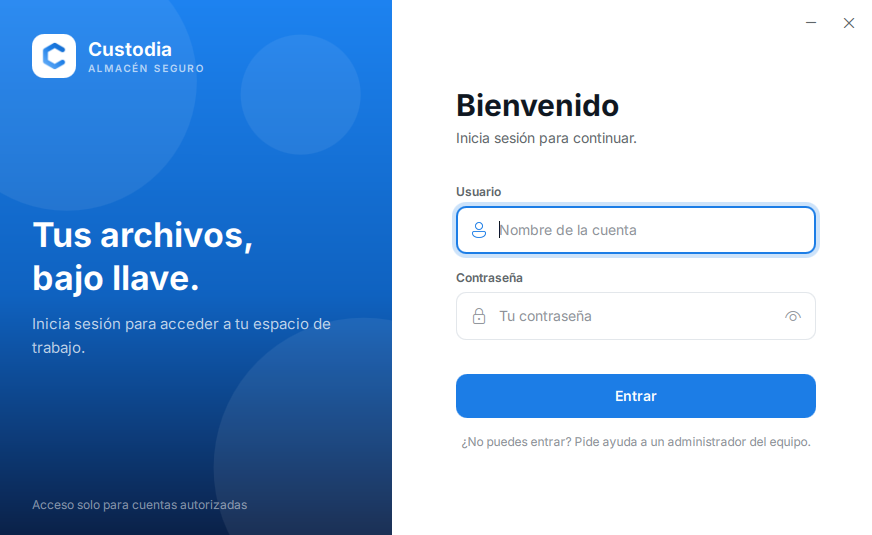
\includegraphics[width=0.49\columnwidth]{figuras/ingreso.png}\hfill
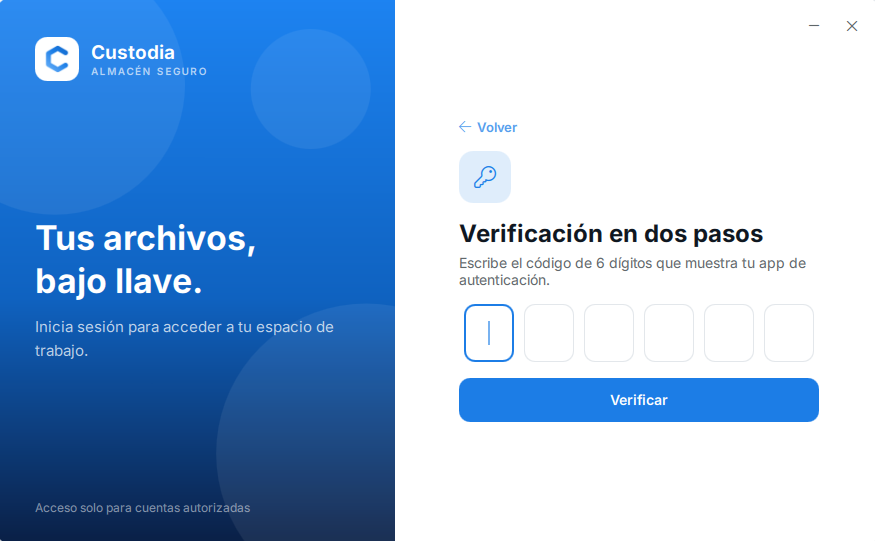
\includegraphics[width=0.49\columnwidth]{figuras/verificacion.png}
\caption{Inicio de sesión (izquierda) y verificación en dos pasos (derecha).}
\label{fig:ingreso}
\end{figure}

\subsection{Activar la verificación en dos pasos}
Es obligatoria para añadir, renombrar, eliminar o exportar archivos y para cambiar permisos. En el perfil (\textbf{Tu cuenta}), abra \textbf{Verificación en dos pasos} y pulse \textbf{Activar}. Escanee el código QR con una aplicación de autenticación del teléfono (Google Authenticator, Microsoft Authenticator u otra compatible), escriba el código que muestra y pulse \textbf{Confirmar y activar}. Si intenta una operación sensible sin haberla activado, Custodia le ofrecerá activarla en ese momento.

\subsection{La ventana principal}
A la izquierda, el panel \textbf{Carpetas} muestra su espacio personal y la carpeta compartida con su grupo; no verá las carpetas de otras personas. Un administrador ve el almacén completo. En el centro, el listado de la carpeta abierta con \textbf{Nombre}, \textbf{Tamaño} y \textbf{Modificado}, y el buscador \textbf{Buscar en esta carpeta}. Sobre el listado, el encabezado indica cuántos elementos hay y cuántos están cifrados. A la derecha, el panel del elemento seleccionado muestra su tipo, tamaño y si está cifrado, su \textbf{Propietario} y, bajo \textbf{Lo que puedes hacer aquí}, sus permisos efectivos: las acciones permitidas aparecen marcadas y las denegadas tachadas. Debajo están las acciones \textbf{Guardar una copia…}, \textbf{Renombrar…} y \textbf{Permisos…}. El ícono de luna, arriba a la derecha, alterna entre tema claro y oscuro (Fig.~\ref{fig:principal}).

\begin{figure}[!htb]
\centering
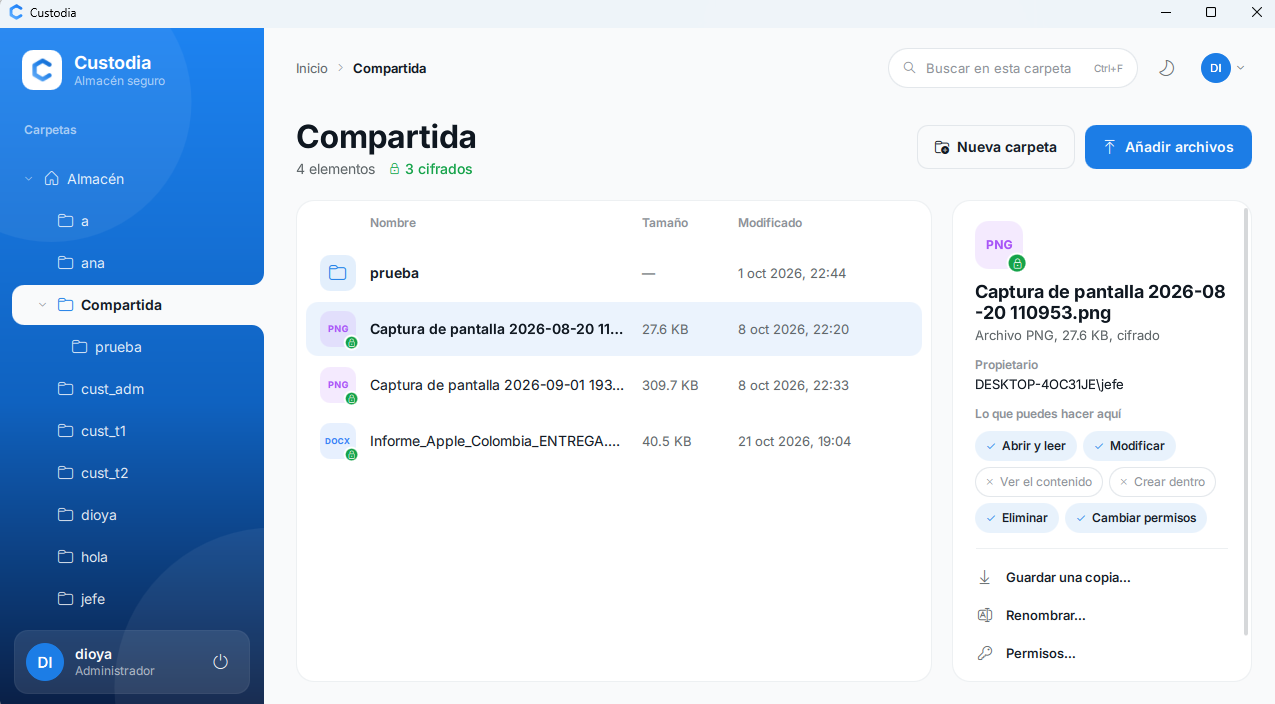
\includegraphics[width=\columnwidth]{figuras/principal.png}
\caption{Ventana principal de un administrador: árbol de carpetas, listado con archivos cifrados y panel de permisos efectivos del archivo seleccionado.}
\label{fig:principal}
\end{figure}


\subsection{Trabajar con archivos}
\begin{itemize}
    \item \textbf{Nueva carpeta}: crea una carpeta en la ubicación actual.
    \item \textbf{Añadir archivos}: guarda uno o varios archivos, cifrados. También puede arrastrarlos a la ventana.
    \item \textbf{Renombrar…} y \textbf{Eliminar}: actúan sobre el elemento seleccionado. Su carpeta personal y la compartida no se pueden renombrar ni eliminar.
    \item \textbf{Guardar una copia…}: exporta una copia legible fuera del almacén. Pide el motivo, que queda en la bitácora (Fig.~\ref{fig:motivo}), y un código de verificación. Se permiten 20 copias cada 10 minutos.
\end{itemize}
Añadir, renombrar, eliminar y guardar una copia piden un código de verificación. Cada código sirve una sola vez: si Custodia responde que ya se usó, espere a que su aplicación muestre uno nuevo (cambia cada 30 segundos). Los códigos incorrectos cuentan para el bloqueo de la cuenta.

\subsection{Permisos}
Seleccione un elemento y pulse \textbf{Permisos…}. La hoja \textbf{Quién tiene acceso} lista las cuentas y grupos con permiso, marcando las entradas \textbf{Heredado} (vienen de la carpeta superior y no se editan aquí) y las de tipo \textbf{Denegado}. En \textbf{Conceder un permiso} escriba la cuenta o el grupo en \textbf{A quién} y elija en \textbf{Qué puede hacer} una o varias opciones: \textbf{Abrir y leer}, \textbf{Modificar}, \textbf{Entrar y recorrer}, \textbf{Eliminar} o \textbf{Control total}. Active \textbf{Aplicar también a lo que contenga} para que las carpetas y archivos de dentro lo hereden, y pulse \textbf{Conceder}. Solo puede cambiar permisos si Windows se lo permite: los administradores y el propietario del elemento (Fig.~\ref{fig:permisos}).

\begin{figure}[!htb]
\centering
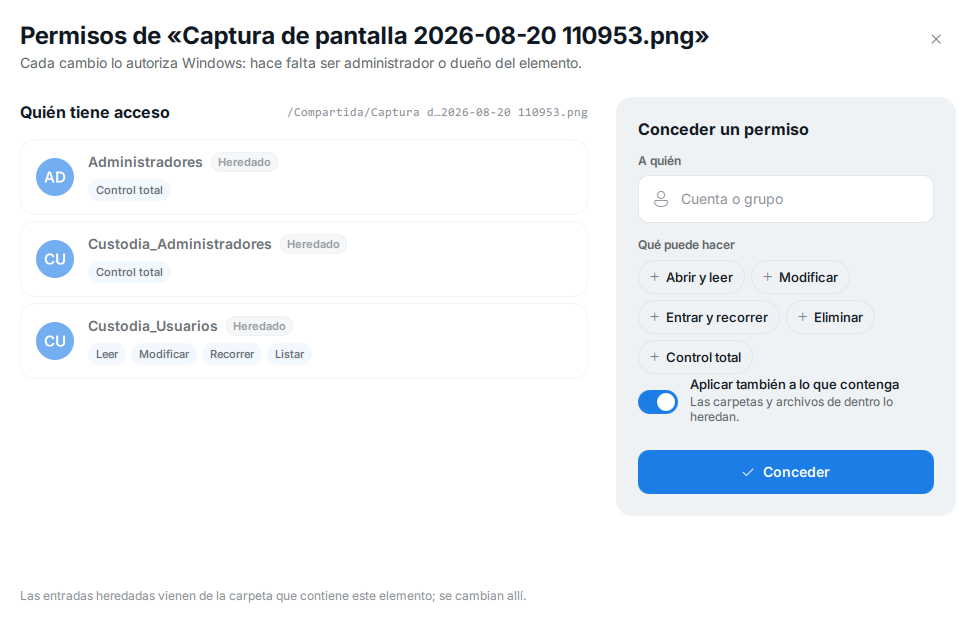
\includegraphics[width=\columnwidth]{figuras/permisos.png}
\caption{Hoja de permisos: entradas heredadas de la carpeta superior y formulario para conceder un permiso.}
\label{fig:permisos}
\end{figure}


\subsection{Cuentas y grupos (administradores)}
Desde \textbf{Cuentas y grupos} (Fig.~\ref{fig:cuentas}) un administrador puede: crear una \textbf{Cuenta nueva}, activando \textbf{Puede administrar Custodia} si la persona debe gestionar cuentas y consultar la bitácora; \textbf{Añadir una cuenta de Windows existente}; \textbf{Asignar a un grupo…} o \textbf{Quitar de un grupo…}; crear un \textbf{Nuevo grupo}; restablecer la contraseña de una persona que la olvidó, con una contraseña temporal que se muestra una sola vez; y restablecer la verificación en dos pasos de quien perdió el teléfono. Las cuentas creadas por Custodia se pueden eliminar; las que ya existían en Windows solo se pueden \textbf{Retirar de Custodia}, sin borrarlas del equipo. Nadie puede retirarse a sí mismo ni retirar al último administrador.

\subsection{Bitácora (administradores)}
La hoja \textbf{Bitácora de auditoría} (Fig.~\ref{fig:bitacora}) muestra los eventos agrupados por día y permite buscar por usuario, recurso o detalle, y filtrar por \textbf{Usuario}, \textbf{Operación}, \textbf{Fecha} (con un calendario que marca los días con actividad) y por resultado: \textbf{Todos}, \textbf{Denegados} o \textbf{Permitidos}. Al elegir un evento se ven todos sus datos. Es de solo lectura: no hay forma de editar ni borrar registros desde la aplicación. El botón \textbf{Verificar integridad} recorre la cadena de registros y la compara con las anclas del Visor de eventos; si algo se alteró, indica desde qué registro y de qué forma. Cada verificación queda también en la bitácora.

\subsection{Respaldo de la clave (administradores)}
Si la clave maestra se pierde o se daña, los archivos cifrados no se pueden abrir, por eso conviene exportar un respaldo apenas se instale Custodia. En el perfil, abra \textbf{Respaldo de la clave} y elija \textbf{Exportar respaldo}: escriba dos veces una contraseña de recuperación de al menos 12 caracteres, elija dónde guardar el archivo \texttt{.custodiakey} (idealmente una USB; Custodia no permite guardarlo en el almacén ni junto a la clave) y confirme con el código de verificación. Quien tenga el archivo y su contraseña puede descifrar todos los archivos: guárdelos en lugares distintos (Fig.~\ref{fig:respaldo}).

\begin{figure}[!htb]
\centering
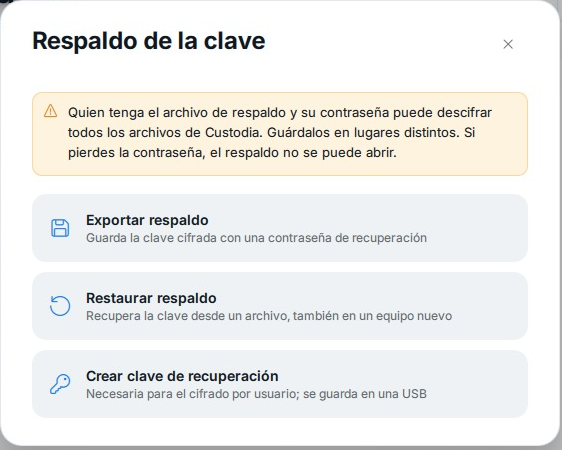
\includegraphics[width=0.86\columnwidth]{figuras/respaldo_menu.png}
\caption{Hoja \textbf{Respaldo de la clave}: exportar, restaurar y crear la clave de recuperación del cifrado por usuario.}
\label{fig:respaldo}
\end{figure}

Para recuperar la clave, entre con una cuenta administradora y use \textbf{Restaurar respaldo}: elija el archivo, escriba la contraseña y confirme con el código. Antes de instalarla, Custodia comprueba que la clave abra los archivos del almacén. Si falta la clave pero hay archivos cifrados, Custodia arranca igual, no genera una clave nueva y deja entrar a un administrador para restaurarla. Con el cifrado por usuario activo, el respaldo guarda a su lado un archivo \texttt{.identidades}: hay que conservar los dos.

\subsection{Cifrado por usuario y clave de recuperación (administradores)}
Con el cifrado por usuario, ni siquiera un administrador puede abrir los archivos personales de otra persona sin su contraseña. Para activarlo, abra \textbf{Respaldo de la clave} y elija \textbf{Crear clave de recuperación} (Fig.~\ref{fig:recuperacion}). Escriba dos veces una contraseña de al menos 12 caracteres, distinta de la del respaldo, y guarde el archivo \texttt{.custodiarec} en una USB. Esta clave se crea una sola vez: la debe guardar el dueño del computador, con una segunda copia en otro lugar. Después se define la variable \texttt{CUSTODIA\_CIFRADO\_POR\_USUARIO=1}; desde entonces, al entrar cada persona sus archivos personales se cifran para ella.

Si alguien olvida su contraseña y un administrador se la restablece, la persona entra pero no puede abrir sus archivos. Con la USB, el administrador elige \textbf{Recuperar archivos de una cuenta} en la misma hoja y se los devuelve. Sin la USB o sin su contraseña, esos archivos se pierden.

\begin{figure}[!htb]
\centering
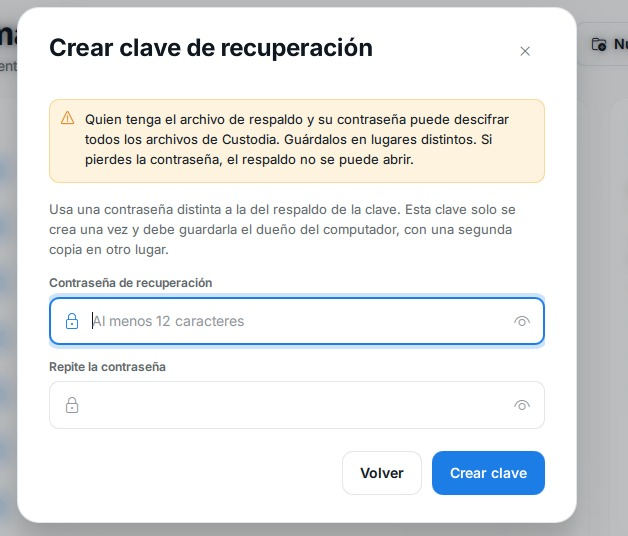
\includegraphics[width=0.8\columnwidth]{figuras/clave_recuperacion.png}
\caption{Creación de la clave de recuperación del cifrado por usuario, que se guarda en una USB con una contraseña propia.}
\label{fig:recuperacion}
\end{figure}

\subsection{Estado del cifrado de disco (administradores)}
Al iniciar, Custodia comprueba si BitLocker protege la unidad donde está el almacén. Si no lo hace, el perfil del administrador muestra \textbf{Volumen sin proteger} con las instrucciones para activarlo (Fig.~\ref{fig:volumen}), y el hallazgo queda en la bitácora. Si se define \texttt{CUSTODIA\_EXIGIR\_BITLOCKER=1}, Custodia no deja entrar mientras la unidad siga sin proteger.

\begin{figure}[!htb]
\centering
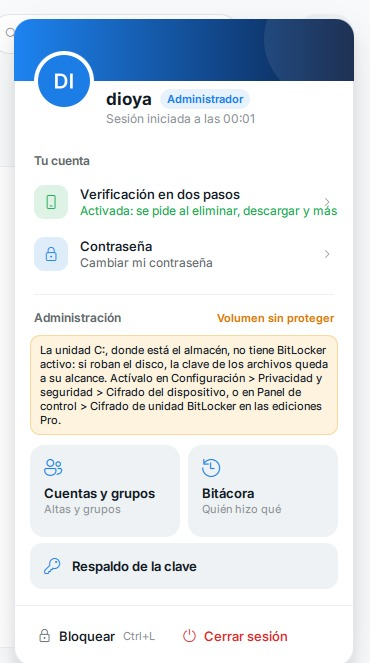
\includegraphics[width=0.5\columnwidth]{figuras/perfil_volumen.png}
\caption{Perfil de un administrador con el aviso de volumen sin proteger.}
\label{fig:volumen}
\end{figure}

\subsection{Bloqueo y cierre de sesión}
Tras 5 minutos sin usar el ratón ni el teclado, o al pulsar Ctrl+L, la ventana se cubre con la pantalla de bloqueo, que muestra la hora y pide su contraseña (Fig.~\ref{fig:bloqueo}). Pulse \textbf{Desbloquear} para continuar o \textbf{Cerrar sesión} para salir. Si permanece bloqueada 30 minutos más, la sesión se cierra. La aplicación permite además cambiar la propia contraseña, alternar entre tema claro y oscuro y cerrar la sesión.

%======================================================================
\section{Resultados y pruebas}
\label{sec:resultados}

\subsection{Estrategia de verificación}
Las pruebas se ejecutan sobre Windows real, no sobre simulaciones: crean cuentas locales temporales, escriben ACL reales y las eliminan al terminar. La prueba central del proyecto (\texttt{test\_el\_kernel\_deniega\_el\_acceso}) suplanta a una cuenta sin permisos e intenta leer un archivo; pasa solo si el rechazo lo emite el núcleo de Windows. Su contraparte comprueba que, al conceder el permiso, la misma operación funciona.

\subsection{Suite de pruebas}
La suite tiene 324 funciones de prueba en veinticuatro archivos; con los casos parametrizados suman 382 pruebas, de las cuales 381 pasan y una se omite (Tabla~\ref{tab:suite}). La cobertura del núcleo, medida con \texttt{pytest-cov}, es del 92~\%.

\begin{table*}[!t]
\caption{Pruebas automatizadas por área}
\label{tab:suite}
\centering
\footnotesize
\setlength{\tabcolsep}{3pt}
\begin{tabular}{|>{\scriptsize}p{3.3cm}|c|p{13.2cm}|}
\hline
\textbf{Archivo} & \textbf{N.º} & \textbf{Qué verifica} \\
\hline
\texttt{test\_cifrado\_\allowbreak usuario} & 60 & Cifrado por usuario sobre Windows real: migración, clave de recuperación, recuperar una cuenta, identidad sustituida que falla cerrada. \\
\hline
\texttt{test\_cadena\_\allowbreak bitacora} & 33 & Cadena íntegra; edición, borrado, inserción y truncado detectados; recálculo frente a las anclas; migración; escritura concurrente. \\
\hline
\texttt{test\_respaldo} & 30 & Respaldo de la clave: ida y vuelta, contraseña incorrecta, archivo alterado, solo administradores, la clave nunca en claro. \\
\hline
\texttt{test\_fsops} & 28 & Operaciones sobre archivos bajo suplantación real: listar, mover, copiar, buscar sin revelar lo vetado. \\
\hline
\texttt{test\_cuentas\_\allowbreak windows} & 28 & Ciclo de vida real de cuentas y grupos de Windows; incorporar y retirar. \\
\hline
\texttt{test\_volumen} & 12 & Estados de BitLocker; bloquea solo si se exige y está confirmado sin proteger; registro y aviso. \\
\hline
\texttt{test\_segundo\-factor} & 11 & Secretos TOTP con DPAPI y ACL reales; fallo cerrado ante blobs dañados o ajenos. \\
\hline
\texttt{test\_auth} & 10 & Sesiones: tokens, expiración, cuentas deshabilitadas, sin enumeración de cuentas. \\
\hline
\texttt{test\_impersonation} & 10 & El núcleo deniega y permite; la identidad se restaura ante excepciones; hilos independientes. \\
\hline
\texttt{test\_permissions} & 10 & Contrato \texttt{can()}; permisos efectivos; la consulta coincide con la operación real. \\
\hline
\texttt{test\_jail} & 10 & Rutas fuera del almacén, flujos alternativos y nombres reservados. \\
\hline
\texttt{test\_crypto} & 10 & Cifrado, \textit{nonce} único, detección de manipulación, clave nunca en claro. \\
\hline
\texttt{test\_accounts} & 10 & Cuentas y grupos; salvaguardas sobre cuentas ajenas e integradas. \\
\hline
\texttt{test\_grupos\_gui} & 9 & Grupos desde la interfaz; último administrador; registro en bitácora. \\
\hline
\texttt{test\_confirmacion} & 7 & Código TOTP por operación, uso único y bloqueo por fallos. \\
\hline
\texttt{test\_contrasenas} & 7 & Contraseñas temporales y cambio obligatorio. \\
\hline
\texttt{test\_alcance} & 6 & Espacios personal y compartido; la raíz no se lista. \\
\hline
\texttt{test\_boveda} & 6 & Cifrado por usuario: solo los destinatarios abren el archivo. \\
\hline
\texttt{test\_totp} & 6 & Vector oficial de la RFC 6238 y tolerancia de reloj. \\
\hline
\texttt{test\_audit} & 5 & Secuencia de RF-05; el usuario registrado es el suplantado. \\
\hline
\texttt{test\_descargas} & 5 & Límite de copias por usuario. \\
\hline
\texttt{test\_seguridad} & 5 & Bloqueo por intentos; mayúsculas no lo evaden. \\
\hline
\texttt{test\_rnf} & 4 & Mediciones de RNF-01, RNF-02 y RNF-05. \\
\hline
\texttt{test\_ingreso\_\allowbreak miembros} & 2 & Solo entran cuentas de Custodia. \\
\hline
\end{tabular}
\end{table*}

\subsection{Requisitos funcionales}
Los trece requisitos funcionales están implementados. Todos excepto RF-11 tienen al menos una prueba automatizada que los verifica (Tabla~\ref{tab:suite}): RF-01 y RF-02 en \texttt{test\_accounts}, \texttt{test\_cuentas\_windows} y \texttt{test\_grupos\_gui}; RF-03 en \texttt{test\_impersonation} y \texttt{test\_fsops}; RF-04 en \texttt{test\_jail}; RF-05 en \texttt{test\_audit} y \texttt{test\_cadena\_bitacora}; RF-06 y RF-07 en \texttt{test\_permissions}; RF-08 en \texttt{test\_crypto}; RF-09 en \texttt{test\_totp}, \texttt{test\_segundofactor} y \texttt{test\_confirmacion}; RF-10 en \texttt{test\_seguridad}; RF-12 en \texttt{test\_descargas} y \texttt{test\_confirmacion}; y RF-13 en \texttt{test\_alcance}. El bloqueo por inactividad (RF-11) depende de eventos de la interfaz y no tiene prueba automatizada.

\subsection{Defectos encontrados por las pruebas}
Las pruebas que llevaron la cobertura del 73~\% al 90~\% se escribieron contra Windows real y no contra simulaciones. Encontraron dos defectos que las pruebas anteriores no detectaban:
\begin{enumerate}
    \item \textbf{Quitar de un grupo y retirar una cuenta fallaban.} La llamada a \texttt{NetLocalGroupDelMembers} pasaba cuatro argumentos y \texttt{pywin32} acepta tres. Las pruebas anteriores de grupos reemplazaban esa función por un doble, por lo que el error nunca se manifestó en ellas.
    \item \textbf{La cuenta no quedaba como propietaria de su espacio.} Asignar otra cuenta como propietaria exige \texttt{SeRestorePrivilege} habilitado, y el error se ocultaba sin registro. Ahora el privilegio se activa solo durante la operación, y un fallo se registra en la bitácora.
\end{enumerate}
Ambos se corrigieron y el ejecutable se reconstruyó con las correcciones. El hallazgo confirma la decisión de probar sobre el sistema operativo real: un doble de prueba solo verifica lo que quien lo escribe supone que hace Windows.

\subsection{Requisitos no funcionales}
La Tabla~\ref{tab:rnfres} presenta las mediciones. Se cumplen seis de los ocho requisitos; RNF-07 se cumple en parte y RNF-04 queda pendiente.

\begin{table}[!t]
\caption{Resultados de los requisitos no funcionales}
\label{tab:rnfres}
\centering
\footnotesize
\setlength{\tabcolsep}{3pt}
\begin{tabular}{|l|p{2.4cm}|p{2.4cm}|p{1.5cm}|}
\hline
\textbf{ID} & \textbf{Criterio} & \textbf{Resultado} & \textbf{Estado} \\
\hline
RNF-01 & 0 suplantaciones remanentes en 100 operaciones & 0 & Cumple \\
\hline
RNF-02 & $\leq$ 500 ms por 10 MB & 49,5 ms & Cumple \\
\hline
RNF-03 & Mismas pruebas en ambos \textit{backends} & Pasan & Cumple \\
\hline
RNF-04 & $\leq$ 3 pasos, 2 personas & Sin realizar & Pendiente \\
\hline
RNF-05 & 0 archivos parciales en 50 denegaciones & 0 & Cumple \\
\hline
RNF-06 & Cobertura $\geq$ 80 \% & 92 \% & Cumple \\
\hline
RNF-07 & Ejecutable único sin Python & Construido (171 MB) con los últimos cambios; falta probarlo en equipo limpio & Cumple en parte \\
\hline
RNF-08 & Sobrecarga $\leq$ 200 ms; clave no en claro & 14,8 ms; clave no aparece & Cumple \\
\hline
\end{tabular}
\end{table}

\subsection{Vectores de ataque}
La Tabla~\ref{tab:vecres} contrasta cada vector con la evidencia obtenida.

\begin{table}[!t]
\caption{Resultado frente a los vectores de ataque}
\label{tab:vecres}
\centering
\footnotesize
\setlength{\tabcolsep}{3pt}
\begin{tabular}{|l|p{4.5cm}|p{1.85cm}|}
\hline
\textbf{ID} & \textbf{Evidencia} & \textbf{Resultado} \\
\hline
V1 & Bloqueo al alcanzar el umbral, también con mayúsculas cambiadas (\texttt{test\_seguridad}). & Mitigado \\
\hline
V2 & Rutas con \texttt{..}, flujos alternativos y nombres reservados rechazadas (\texttt{test\_jail}). & Mitigado \\
\hline
V3 & El núcleo deniega sin ACE; la raíz no se enumera (\texttt{test\_impersonation}, \texttt{test\_alcance}). & Mitigado \\
\hline
V4 & Identidad restaurada ante excepciones y en 100 operaciones (\texttt{test\_rnf}). & Mitigado \\
\hline
V5 & El archivo en disco no es legible (\texttt{test\_crypto}); un volumen sin BitLocker se detecta y puede impedir la entrada (\texttt{test\_volumen}). & Mitigado en parte \\
\hline
V6 & La clave no está en claro en disco; con el cifrado por usuario activo, obtenerla de DPAPI ya no abre los archivos personales (\texttt{test\_cifrado\_usuario}). & Mitigado si se activa C20 \\
\hline
V7 & Un byte alterado hace fallar el descifrado (\texttt{test\_crypto}). & Mitigado \\
\hline
V8 & El usuario suplantado no escribe la bitácora (\texttt{test\_audit}); lo que altere un administrador se detecta (\texttt{test\_cadena\_bitacora}). & Mitigado (detección) \\
\hline
V9 & Respaldo exportable y restauración verificada (\texttt{test\_respaldo}); falta probarla en un segundo equipo físico. & Mitigado \\
\hline
V10 & Sin servicio de red; no se probó un ataque de carga de bibliotecas. & Sin prueba \\
\hline
V11 & Código TOTP por operación y de uso único (\texttt{test\_confirmacion}); bloqueo por inactividad sin prueba automatizada. & Mitigado \\
\hline
V12 & Límite de copias por usuario (\texttt{test\_descargas}). & Mitigado \\
\hline
\end{tabular}
\end{table}

%======================================================================
\section{Conclusiones y recomendaciones}
\label{sec:conclusiones}

\subsection{Conclusiones}
\begin{itemize}
    \item \textbf{Los tres objetivos específicos se cumplieron.} Los archivos se cifran con AES-256-GCM; la autorización la decide Windows, y una prueba sobre el sistema real lo demuestra; y cada operación intentada queda en una bitácora que el usuario auditado no puede alterar y cuya alteración por un administrador queda en evidencia.
    \item \textbf{Delegar la autorización eliminó el riesgo más alto del caso.} El acceso de un usuario a archivos ajenos pasó de crítico a bajo sin escribir una sola regla de permisos en la aplicación.
    \item \textbf{La implementación reveló riesgos que el diseño no veía.} La sesión desatendida y la exportación de copias legibles (R15, R16) aparecieron al usar la aplicación, no en el papel, y motivaron cinco requisitos nuevos. El análisis de riesgos resultó ser un proceso continuo y no un entregable cerrado.
    \item \textbf{El rendimiento no fue una restricción.} Suplantar y cifrar en cada operación cuesta decenas de milisegundos, un orden de magnitud por debajo de los límites fijados.
    \item \textbf{Probar contra el sistema real encontró lo que las simulaciones ocultaban.} Dos defectos de administración de cuentas solo aparecieron cuando las pruebas usaron Windows de verdad.
    \item \textbf{Los riesgos altos que quedan dependen de la configuración.} El robo del disco completo (R1) y un administrador local que pida la clave a DPAPI (R6) siguen altos con la configuración por defecto. Con BitLocker exigido y el cifrado por usuario activo bajan a nivel medio y no queda ningún riesgo alto.
\end{itemize}

\subsection{Recomendaciones}
\begin{enumerate}
    \item Exportar el respaldo de la clave apenas se instale Custodia, guardar el archivo y su contraseña en lugares distintos, y probar la restauración en un segundo equipo físico~\cite{sp80057}.
    \item Activar BitLocker con TPM en el equipo anfitrión y definir \texttt{CUSTODIA\_EXIGIR\_BITLOCKER=1}, para cubrir el robo del disco completo (R1).
    \item Realizar la prueba de usabilidad con dos personas ajenas al desarrollo (RNF-04).
    \item Probar el ejecutable en un equipo limpio y reducir su tamaño excluyendo los módulos de Qt que no se usan.
    \item Sincronizar el reloj del equipo y dar al registro Application del Visor de eventos un tamaño suficiente, o reenviarlo a otro equipo, para que las anclas de la bitácora (C16) no se pierdan por rotación ni por un administrador local.
    \item Crear la clave de recuperación y activar el cifrado por usuario (C20); cuando no queden archivos con clave maestra fuera de la carpeta compartida, dejarlo activo por defecto (R6).
    \item Si se despliega con datos personales reales, documentar el tratamiento conforme a la Ley 1581 de 2012.
\end{enumerate}

\begin{thebibliography}{00}
\raggedright
\bibitem{fips197} National Institute of Standards and Technology, \textit{Advanced Encryption Standard (AES)}, FIPS PUB 197, nov. 2001.
\bibitem{msacl} Microsoft, ``Access control lists,'' Microsoft Learn. [En línea]. Disponible: \url{https://learn.microsoft.com/windows/win32/secauthz/access-control-lists} (accedido: 6 nov. 2026).
\bibitem{msimp} Microsoft, ``ImpersonateLoggedOnUser function (securitybaseapi.h),'' Microsoft Learn. [En línea]. Disponible: \url{https://learn.microsoft.com/windows/win32/api/securitybaseapi/nf-securitybaseapi-impersonateloggedonuser} (accedido: 6 nov. 2026).
\bibitem{saltzer} J. H. Saltzer y M. D. Schroeder, ``The protection of information in computer systems,'' \textit{Proc. IEEE}, vol. 63, n.º 9, pp. 1278--1308, sep. 1975, doi: 10.1109/PROC.1975.9939.
\bibitem{sandhu} R. S. Sandhu y P. Samarati, ``Access control: Principle and practice,'' \textit{IEEE Commun. Mag.}, vol. 32, n.º 9, pp. 40--48, sep. 1994, doi: 10.1109/35.312842.
\bibitem{lampson} B. W. Lampson, ``Protection,'' \textit{ACM SIGOPS Oper. Syst. Rev.}, vol. 8, n.º 1, pp. 18--24, ene. 1974.
\bibitem{winint} P. Yosifovich, A. Ionescu, M. E. Russinovich y D. A. Solomon, \textit{Windows Internals, Part 1}, 7.ª ed. Redmond, WA, USA: Microsoft Press, 2017.
\bibitem{mslogon} Microsoft, ``LogonUserW function (winbase.h),'' Microsoft Learn. [En línea]. Disponible: \url{https://learn.microsoft.com/windows/win32/api/winbase/nf-winbase-logonuserw} (accedido: 6 nov. 2026).
\bibitem{daemen} J. Daemen y V. Rijmen, \textit{The Design of Rijndael: AES --- The Advanced Encryption Standard}. Berlín, Alemania: Springer, 2002.
\bibitem{nist38d} M. Dworkin, \textit{Recommendation for Block Cipher Modes of Operation: Galois/Counter Mode (GCM) and GMAC}, NIST Special Publication 800-38D, nov. 2007.
\bibitem{mcgrew} D. A. McGrew y J. Viega, ``The security and performance of the Galois/Counter Mode (GCM) of operation,'' en \textit{Progress in Cryptology -- INDOCRYPT 2004}, ser. LNCS, vol. 3348. Berlín, Alemania: Springer, 2004, pp. 343--355, doi: 10.1007/978-3-540-30556-9\_27.
\bibitem{msdpapi} Microsoft, ``CryptProtectData function (dpapi.h),'' Microsoft Learn. [En línea]. Disponible: \url{https://learn.microsoft.com/windows/win32/api/dpapi/nf-dpapi-cryptprotectdata} (accedido: 6 nov. 2026).
\bibitem{sp80057} E. Barker, \textit{Recommendation for Key Management: Part 1 -- General}, NIST Special Publication 800-57 Part 1 Rev. 5, may. 2020.
\bibitem{rfc8017} K. Moriarty, B. Kaliski, J. Jonsson y A. Rusch, ``PKCS \#1: RSA Cryptography Specifications Version 2.2,'' IETF, RFC 8017, nov. 2016.
\bibitem{rfc7914} C. Percival y S. Josefsson, ``The scrypt Password-Based Key Derivation Function,'' IETF, RFC 7914, ago. 2016.
\bibitem{bonneau} J. Bonneau, C. Herley, P. C. van Oorschot y F. Stajano, ``The quest to replace passwords: A framework for comparative evaluation of web authentication schemes,'' en \textit{Proc. IEEE Symp. Security and Privacy}, San Francisco, CA, USA, 2012, pp. 553--567, doi: 10.1109/SP.2012.44.
\bibitem{ometov} A. Ometov, S. Bezzateev, N. Mäkitalo, S. Andreev, T. Mikkonen y Y. Koucheryavy, ``Multi-factor authentication: A survey,'' \textit{Cryptography}, vol. 2, n.º 1, art. 1, ene. 2018, doi: 10.3390/cryptography2010001.
\bibitem{rfc4226} D. M'Raihi, M. Bellare, F. Hoornaert, D. Naccache y O. Ranen, ``HOTP: An HMAC-Based One-Time Password Algorithm,'' IETF, RFC 4226, dic. 2005.
\bibitem{rfc6238} D. M'Raihi, S. Machani, M. Pei y J. Rydell, ``TOTP: Time-Based One-Time Password Algorithm,'' IETF, RFC 6238, may. 2011.
\bibitem{sp80063b} P. A. Grassi \textit{et al.}, \textit{Digital Identity Guidelines: Authentication and Lifecycle Management}, NIST Special Publication 800-63B, jun. 2017.
\bibitem{iso27001} \textit{Information security, cybersecurity and privacy protection --- Information security management systems --- Requirements}, ISO/IEC 27001:2022.
\bibitem{sp80092} K. Kent y M. Souppaya, \textit{Guide to Computer Security Log Management}, NIST Special Publication 800-92, sep. 2006.
\bibitem{sp80086} K. Kent, S. Chevalier, T. Grance y H. Dang, \textit{Guide to Integrating Forensic Techniques into Incident Response}, NIST Special Publication 800-86, ago. 2006.
\bibitem{iso27037} \textit{Information technology --- Security techniques --- Guidelines for identification, collection, acquisition and preservation of digital evidence}, ISO/IEC 27037:2012.
\bibitem{schneier} B. Schneier y J. Kelsey, ``Secure audit logs to support computer forensics,'' \textit{ACM Trans. Inf. Syst. Secur.}, vol. 2, n.º 2, pp. 159--176, may. 1999, doi: 10.1145/317087.317089.
\bibitem{garfinkel} S. L. Garfinkel, ``Digital forensics research: The next 10 years,'' \textit{Digit. Investig.}, vol. 7, pp. S64--S73, ago. 2010, doi: 10.1016/j.diin.2010.05.009.
\bibitem{magerit1} Ministerio de Hacienda y Administraciones Públicas, \textit{MAGERIT versión 3.0: Metodología de Análisis y Gestión de Riesgos de los Sistemas de Información. Libro I: Método}. Madrid, España, 2012.
\bibitem{magerit2} Ministerio de Hacienda y Administraciones Públicas, \textit{MAGERIT versión 3.0. Libro II: Catálogo de Elementos}. Madrid, España, 2012.
\bibitem{iso27005} \textit{Information security, cybersecurity and privacy protection --- Guidance on managing information security risks}, ISO/IEC 27005:2022.
\bibitem{ley1581} Congreso de la República de Colombia, ``Ley Estatutaria 1581 de 2012, por la cual se dictan disposiciones generales para la protección de datos personales,'' \textit{Diario Oficial}, n.º 48.587, 18 oct. 2012.
\bibitem{ley1273} Congreso de la República de Colombia, ``Ley 1273 de 2009, por medio de la cual se modifica el Código Penal, se crea un nuevo bien jurídico tutelado denominado `de la protección de la información y de los datos','' \textit{Diario Oficial}, n.º 47.223, 5 ene. 2009.
\bibitem{pytestcov} pytest-cov contributors, ``pytest-cov documentation.'' [En línea]. Disponible: \url{https://pytest-cov.readthedocs.io} (accedido: 6 nov. 2026).
\bibitem{sqlite} SQLite Consortium, ``SQLite documentation.'' [En línea]. Disponible: \url{https://www.sqlite.org/docs.html} (accedido: 6 nov. 2026).
\bibitem{pyside} The Qt Company, ``Qt for Python documentation.'' [En línea]. Disponible: \url{https://doc.qt.io/qtforpython-6/} (accedido: 6 nov. 2026).
\bibitem{pyinstaller} PyInstaller Development Team, ``PyInstaller manual.'' [En línea]. Disponible: \url{https://pyinstaller.org} (accedido: 6 nov. 2026).
\bibitem{stride} A. Shostack, \textit{Threat Modeling: Designing for Security}. Indianapolis, IN, USA: Wiley, 2014.
\bibitem{attack} The MITRE Corporation, ``MITRE ATT\&CK.'' [En línea]. Disponible: \url{https://attack.mitre.org} (accedido: 6 nov. 2026).
\bibitem{cwe} The MITRE Corporation, ``Common Weakness Enumeration (CWE).'' [En línea]. Disponible: \url{https://cwe.mitre.org} (accedido: 6 nov. 2026).
\bibitem{pyca} Python Cryptographic Authority, ``cryptography documentation.'' [En línea]. Disponible: \url{https://cryptography.io} (accedido: 6 nov. 2026).
\bibitem{pywin32} M. Hammond \textit{et al.}, ``pywin32: Python for Windows Extensions.'' [En línea]. Disponible: \url{https://github.com/mhammond/pywin32} (accedido: 6 nov. 2026).
\bibitem{segno} L. Heuer, ``Segno: Python QR Code and Micro QR Code encoder.'' [En línea]. Disponible: \url{https://segno.readthedocs.io} (accedido: 6 nov. 2026).
\bibitem{repo} D. Y. Aranguren Sanabria y P. A. Quintana Barrera, ``Custodia: código fuente,'' GitHub, 2026. [En línea]. Disponible: \url{https://github.com/yanni2327/custodia}
\end{thebibliography}

%======================================================================
\appendices
\section{Comandos de verificación}
\label{anx:comandos}
Cualquier auditor puede comprobar con herramientas de Windows, sin pasar por Custodia, que los controles son reales. Desde una consola como administrador:
\begin{itemize}
    \item \texttt{net localgroup Custodia\_Usuarios}: cuentas dadas de alta en la aplicación.
    \item \texttt{net user <cuenta>}: grupos y estado de una cuenta.
    \item \texttt{icacls} \path{C:\ProgramData\Custodia\storage}: permisos de la raíz del almacén, que para los usuarios solo deben permitir atravesarla.
    \item \texttt{icacls} \path{C:\ProgramData\Custodia\master.key}: acceso limitado a Administradores y SYSTEM.
    \item Abrir cualquier archivo del almacén con un editor de texto: debe empezar con \texttt{CUSTODIA} seguido de contenido ilegible.
    \item \texttt{manage-bde -status C:}: estado de BitLocker en la unidad del almacén, el mismo que comprueba Custodia (C15).
    \item Visor de eventos, registro Application, origen \texttt{Custodia}: anclas de la bitácora con el último id y su resumen (C16).
\end{itemize}

\section{Matriz de trazabilidad}
\label{anx:trazabilidad}
La Tabla~\ref{tab:traza} relaciona cada requisito funcional con los controles que lo implementan (Tabla~\ref{tab:controles}) y con las pruebas automatizadas que lo verifican (Tabla~\ref{tab:suite}). Permite comprobar que ningún requisito queda sin control y señala el único que carece de prueba automatizada.

\begin{table}[!htb]
\caption{Trazabilidad entre requisitos, controles y pruebas}
\label{tab:traza}
\centering
\footnotesize
\setlength{\tabcolsep}{3pt}
\begin{tabular}{|l|p{1.6cm}|>{\raggedright\arraybackslash}p{4.6cm}|}
\hline
\textbf{Req.} & \textbf{Controles} & \textbf{Pruebas} \\
\hline
RF-01 & C1, C21 & \texttt{test\_accounts}, \texttt{test\_cuentas\_windows} \\
\hline
RF-02 & C4, C21 & \texttt{test\_accounts}, \texttt{test\_grupos\_gui} \\
\hline
RF-03 & C3, C6, C11 & \texttt{test\_impersonation}, \texttt{test\_fsops}, \texttt{test\_rnf} \\
\hline
RF-04 & C5 & \texttt{test\_jail} \\
\hline
RF-05 & C7, C12, C16 & \texttt{test\_audit}, \texttt{test\_cadena\_bitacora} \\
\hline
RF-06 & C3 & \texttt{test\_permissions} \\
\hline
RF-07 & C3 & \texttt{test\_permissions} \\
\hline
RF-08 & C8, C9, C10 & \texttt{test\_crypto} \\
\hline
RF-09 & C17 & \texttt{test\_totp}, \texttt{test\_segundofactor}, \texttt{test\_confirmacion} \\
\hline
RF-10 & C2 & \texttt{test\_seguridad} \\
\hline
RF-11 & C18 & Sin prueba automatizada \\
\hline
RF-12 & C19 & \texttt{test\_descargas}, \texttt{test\_confirmacion} \\
\hline
RF-13 & C4 & \texttt{test\_alcance} \\
\hline
C13\,$^{*}$ & C13 & \texttt{test\_respaldo} \\
\hline
C15\,$^{*}$ & C15 & \texttt{test\_volumen} \\
\hline
C20\,$^{*}$ & C20 & \texttt{test\_boveda}, \texttt{test\_cifrado\_usuario} \\
\hline
\multicolumn{3}{|l|}{\scriptsize $^{*}$ Controles sin requisito funcional propio.} \\
\hline
\end{tabular}
\end{table}

\section{Capturas de pantalla}
\label{anx:capturas}
Las Figs.~\ref{fig:cuentas} a~\ref{fig:motivo} complementan las del manual de usuario (Sección~\ref{sec:manual}). Se tomaron con cuentas de prueba creadas por las autoras.

\begin{figure}[H]
\centering
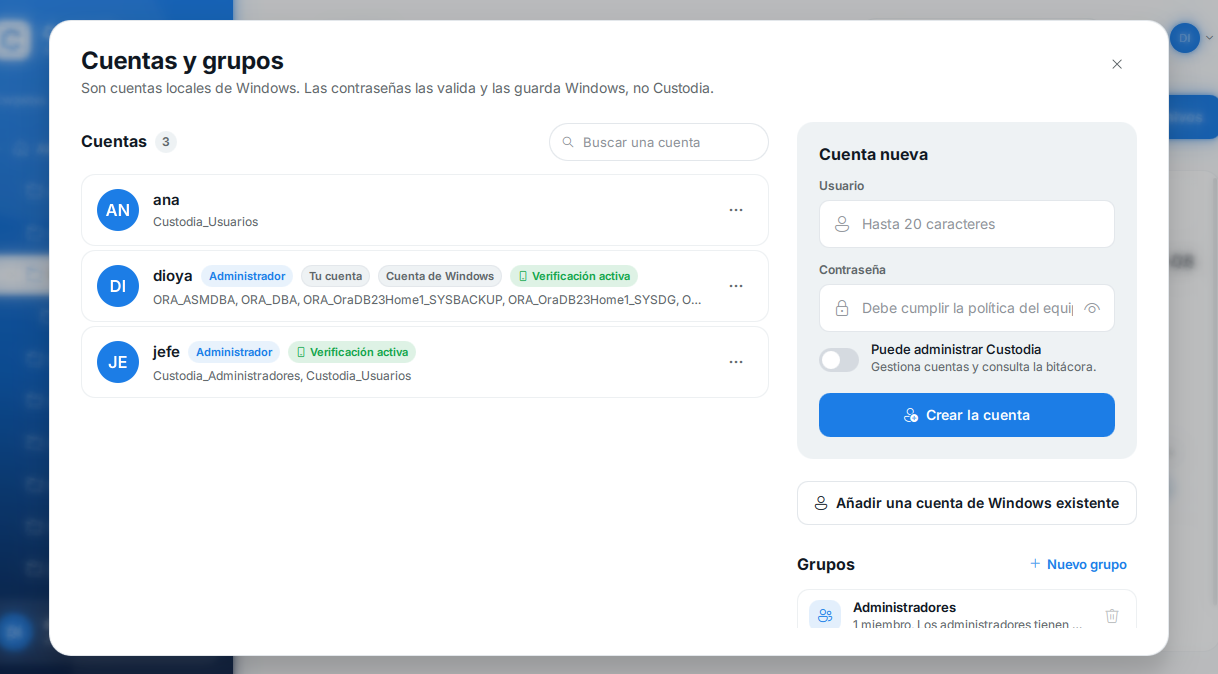
\includegraphics[width=\columnwidth]{figuras/cuentas.png}
\caption{Hoja de cuentas y grupos. Cada cuenta indica su rol, si es una cuenta de Windows incorporada y si tiene la verificación en dos pasos activa.}
\label{fig:cuentas}
\end{figure}

\begin{figure}[H]
\centering
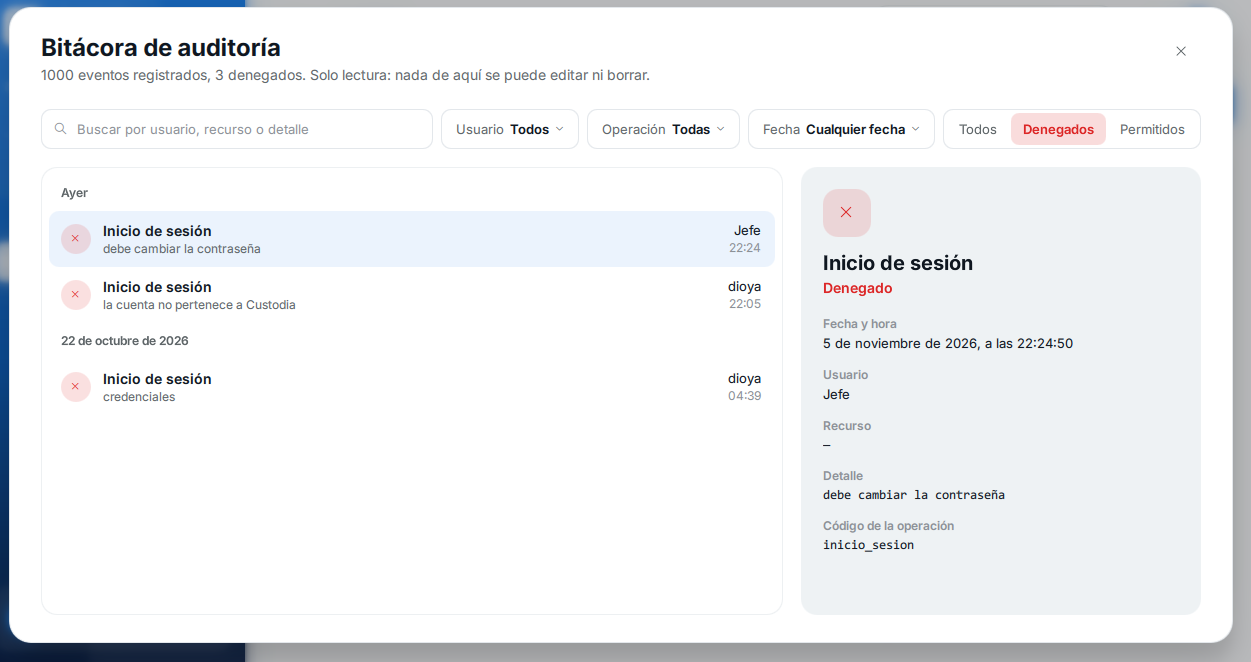
\includegraphics[width=\columnwidth]{figuras/bitacora.png}
\caption{Bitácora de auditoría filtrada por eventos denegados, con el detalle de un inicio de sesión rechazado porque la cuenta debía cambiar su contraseña.}
\label{fig:bitacora}
\end{figure}

\begin{figure}[H]
\centering
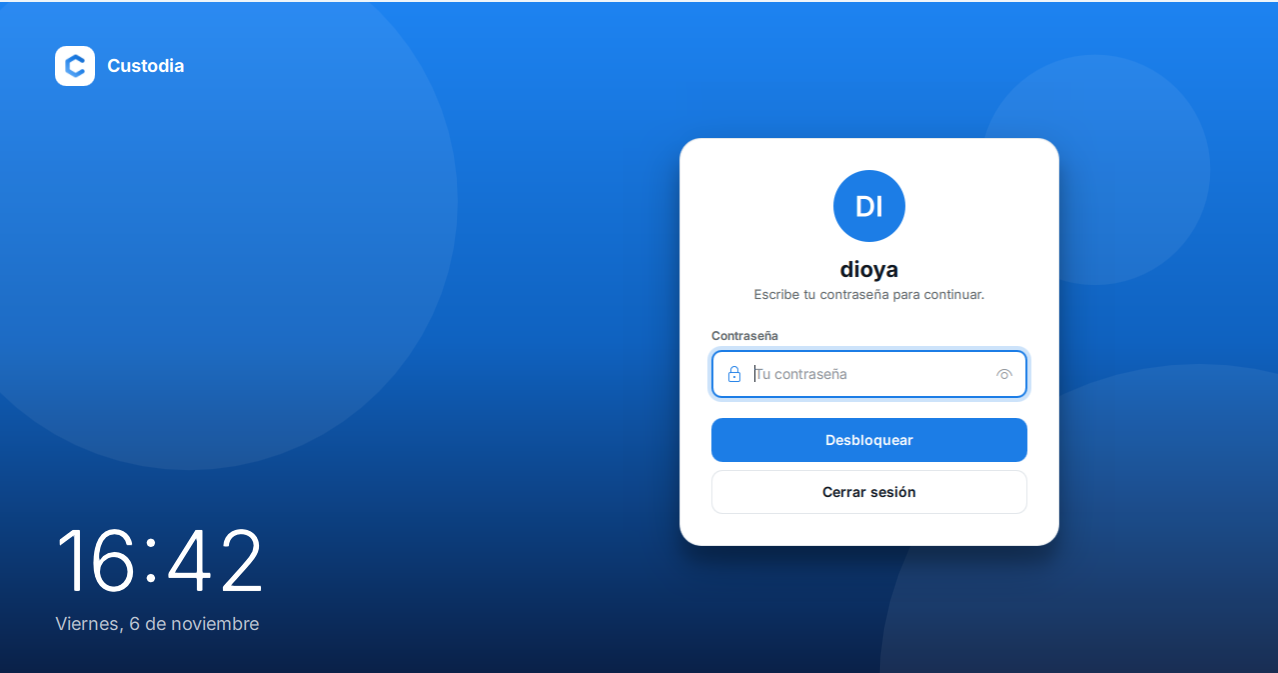
\includegraphics[width=\columnwidth]{figuras/bloqueo.png}
\caption{Pantalla de bloqueo por inactividad.}
\label{fig:bloqueo}
\end{figure}

\begin{figure}[H]
\centering
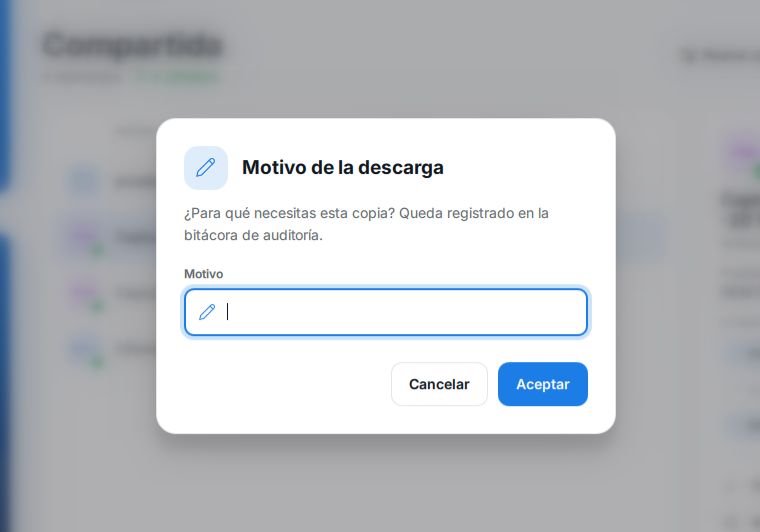
\includegraphics[width=0.72\columnwidth]{figuras/motivo.png}
\caption{Motivo obligatorio antes de exportar una copia; queda registrado en la bitácora.}
\label{fig:motivo}
\end{figure}

\section{Cronología de la implementación}
\label{anx:cronologia}
La Tabla~\ref{tab:crono} reconstruye las etapas a partir de la fecha de última modificación de los archivos del proyecto.

\begin{table}[!htb]
\caption{Etapas de la implementación}
\label{tab:crono}
\centering
\footnotesize
\begin{tabular}{|p{1.4cm}|p{6.5cm}|}
\hline
\textbf{Fecha} & \textbf{Trabajo} \\
\hline
8 oct. 2026 & Núcleo: suplantación, cuentas, ACL, confinamiento, permisos, cifrado y bitácora, con sus pruebas. \\
\hline
20 oct. 2026 & Bloqueo por intentos, control de copias y cifrado por usuario. \\
\hline
21--22 oct. 2026 & Espacios personal y compartido; nueva pantalla de ingreso. \\
\hline
5 nov. 2026 & Interfaz completa en QML; verificación en dos pasos y confirmación de operaciones; contraseñas temporales; gestión de grupos; bloqueo por inactividad. \\
\hline
6 nov. 2026 & Icono, receta de empaquetado, ejecutable \texttt{Custodia.exe} y documentación. \\
\hline
9 nov. 2026 & Respaldo y recuperación de la clave maestra (C13); pruebas nuevas que llevan la cobertura al 90~\%; corrección de los dos defectos que encontraron; nuevo ejecutable. \\
\hline
10 nov. 2026 & Bitácora encadenada y anclada en el Visor de eventos (C16); comprobación de BitLocker (C15); clave de recuperación y migración al cifrado por usuario (C20); cobertura del 92~\%; nuevo ejecutable. \\
\hline
\end{tabular}
\end{table}

\end{document}
